\subsection{生成模与有限生成投射模}

命题 2. —— 设 A 与 B 是 k 上代数，P 是一个 \((A,B)_{k}\)-双模。假设映射 \(b \mapsto b_{P}\)（从 B 到 \(\operatorname{End}_{\mathrm{A}}(\mathrm{P})\)）是双射。下列断言等价：

\begin{enumerate}
\def\labelenumi{(\roman{enumi})}
\item
  A-模 P 是投射的且有限生成的。
\item
  映射 \(\Theta\)（VIII, 第 96 页）是一个 \((\mathrm{B},\mathrm{B})_k\)-双模同构，从 \(\mathrm{P}^* \otimes_{\mathrm{A}} \mathrm{P}\) 到 \(s\mathrm{B}_d\)。
\item
  \(\Theta\) 的像含有 B 的单位元。
\end{enumerate}

此外，若映射 \(a \mapsto a_{P}\)（从 A 到 \(\operatorname{End}_{\mathrm{B}}(\mathrm{P})\)）是双射，则上述断言等价于下述命题：

\begin{enumerate}
\def\labelenumi{(\roman{enumi})}
\setcounter{enumi}{3}
\tightlist
\item
  存在一个 \((\mathrm{B},\mathrm{A})_{k}\)-双模 Q 和一个 \((\mathrm{B},\mathrm{B})_{k}\)-双模满同态，从 \(Q\otimes_{A}P\) 到 \(_{s}B_{d}\)。
\end{enumerate}

由 II, §4, No.~2, 第 271 页的推论，断言 (i) 蕴含 (ii)。此外，(iii) 由 (ii) 得出。设 \(t \in \mathrm{B}^* \otimes_{\mathrm{A}} \mathrm{B}\) 满足 \(\Theta(t) = 1\)。设 \(n\) 是一个整数，并设 \((x_1, \ldots, x_n) \in \mathrm{P}^n\) 与 \((x_1^*, \ldots, x_n^*) \in \mathrm{P}^{*n}\) 满足 \(t = \sum_{i=1}^{n} x_i^* \otimes x_i\)。对每个 \(x\)（属于 \(\mathrm{P}\)），关系式 \(x\Theta(t) = x\) 可以写成

\[
\sum_ {i = 1} ^ {n} \langle x, x _ {i} ^ {*} \rangle x _ {i} = x.
\]

由此推出 A-模 P 由族 \((x_{i})_{1\leqslant i\leqslant n}\) 有限生成，而蕴含关系 (iii) \(\Rightarrow\) (i) 的证明可借助 II, §2, No.~6, 第 238 页的命题 12 完成。

我们显然有 (ii) \(\Rightarrow\) (iv)。设 \(Q\) 是一个 \((B,A)_k\)-双模，\(\theta\) 是一个 \((B,B)_k\)-双模满同态，从 \(Q \otimes_A P\) 到 \(s B_d\)。沿用上一小节的记号，存在一个 \((B,A)_k\)-双模的同态 \(\zeta: Q \to \widetilde{P}\)，使得 \(\theta(y \otimes x) = \langle \zeta(y), x \rangle\)（对 \(x \in P\) 与 \(y \in Q\)），且我们有 \(\theta = \widetilde{\Lambda} \circ (\zeta \otimes 1_P)\)。由于 \(\theta\) 是满射，\(\widetilde{\Lambda}\) 亦然。若映射 \(a \mapsto a_P\)（从 \(A\) 到 \(\mathrm{End}_B(P)\)）是双射，则由 VIII, 第 97 页命题 1 的关系式 (14)，\(\Theta\) 是满射；于是得到蕴含关系 (iv) \(\Rightarrow\) (iii)。

命题 3. —— 设 A 与 B 是 k 上代数，P 是一个 \((A,B)_{k}\)-双模。下列性质等价：

\begin{enumerate}
\def\labelenumi{(\roman{enumi})}
\item
  A-模 P 是生成模。
\item
  映射 \(\Lambda\)（从 \(\mathrm{P} \otimes_{\mathrm{B}} \mathrm{P}^{*}\) 到 \(s\mathrm{A}_{d}\)，VIII, 第 95 页）的像含有单位元。
\item
  存在一个 \((\mathrm{B},\mathrm{A})_{k}\)-双模 Q 和一个 \((\mathrm{A},\mathrm{A})_{k}\)-双模满同态，从 \(P\otimes_{B}Q\) 到 \(_{s}A_{d}\)。
\end{enumerate}

此外，若映射 \(b \mapsto b_{P}\)（从 B 到 \(\operatorname{End}_{\mathrm{A}}(\mathrm{P})\)）是双射，则这些断言等价于下述命题：

\begin{enumerate}
\def\labelenumi{(\roman{enumi})}
\setcounter{enumi}{3}
\tightlist
\item
  映射 \(\Lambda\) 是从 \(\mathrm{P} \otimes_{\mathrm{B}} \mathrm{P}^{*}\) 到 \(s\mathrm{A}_d\) 的同构。
\end{enumerate}

(i) \(\Leftrightarrow\) (ii)：\(\Lambda\) 的像是迹理想 \(\tau(\mathrm{P})\)（VIII, 第 80 页）。于是 (i) 与 (ii) 的等价性由 VIII, 第 80 页的定理 1 得出。

(ii) \(\Rightarrow\) (iii)：只需取 \(Q = P^{*}\)。

(iii) \(\Rightarrow\) (ii)：设 \(Q\) 是一个 \((B,A)_k\)-双模，\(\psi\) 是一个 \((A,A)_k\)-双模同态，从 \(P \otimes_B Q\) 到 \({}_s A_d\)。存在一个 \((B,A)_k\)-双模同态 \(\Psi\)，从 \(Q\) 到 \(P^*\)，使得 \(\psi(x \otimes y) = \langle x, \Psi(y) \rangle\)（对 \(x \in P\) 与 \(y \in Q\)），且我们有等式 \(\psi = \Lambda \circ (1_P \otimes \Psi)\)。若 \(\psi\) 是满射，则 \(\Lambda\) 亦然。

显然 (iv) 蕴含 (ii)。反之，设性质 (ii) 成立，且映射 \(b \mapsto b_{P}\)（从 B 到 \(\operatorname{End}_{\mathrm{A}}(\mathrm{P})\)）是双射。设 e 是 \(P \otimes_{B} P^{*}\) 中满足 \(\Lambda(e) = 1\) 的元素。由 VIII, 第 96 页的关系式 (7)，有 \(u = \Lambda(u)e\)（对 \(P \otimes_{B} P^{*}\) 中的每个 u）；由此得到 \(\Lambda\) 的单射性。

命题 4. —— 设 A 与 B 是 k-代数，P 是一个 \((\mathrm{A},\mathrm{B})_{k}\)-双模。假设映射 \(b\mapsto b_{P}\)（从 B 到 \(\operatorname{End}_{\mathrm{A}}(\mathrm{P})\)）是双射。

\begin{enumerate}
\def\labelenumi{\alph{enumi})}
\item
  若 A-模 P 是生成模，则右 B-模 P 是投射的且有限生成的。
\item
  若 A-模 P 是投射的且有限生成的，则右 B-模 P 是生成模。
\end{enumerate}

设 A-模 P 是生成模。于是它是忠实的且平衡的（VIII, 第 82 页，定理 2），因而映射 \(a \mapsto a_{\mathrm{P}}\)（从 A 到 \(\mathrm{End}_{\mathrm{B}}(\mathrm{P})\)）是双射（VIII, 第 97 页，注 1）。此外，映射 \(\Lambda : \mathrm{P} \otimes_{\mathrm{B}} \mathrm{P}^{*} \to {}_{s} \mathrm{A}_{d}\) 是双射（VIII, 第 98 页，命题 3）。我们把 P 视为 \((\mathrm{B}^{\circ}, \mathrm{A}^{\circ})_{k}\)-双模。映射 \(\Lambda\) 诱导出双射 \(\mathrm{P}^{*} \otimes_{\mathrm{B}^{\circ}} \mathrm{P} \to \mathrm{A}^{\circ}\)；由 VIII, 第 98 页命题 2 的 (iv) \(\Rightarrow\) (i)，右 B-模 P 是投射的且有限生成的。

现在设 A-模 P 是投射的且有限生成的。于是映射 \(\Theta: P^{*} \otimes_{A} P \to_{s} B_{d}\) 是双射（同前所引，(i) \(\Rightarrow\) (ii)）。把上面的命题 3 的蕴含关系 (iii) \(\Rightarrow\) (i) 应用于 \((\mathrm{B}^{\circ}, \mathrm{A}^{\circ})_{k}\)-双模 P，即知右 B-模 P 是生成模。

推论 1. —— 生成模的反模是投射的且有限生成的。有限生成投射模的反模是生成模。

设 A 是一个 k-代数，M 是一个 A-模。用 B 表示代数 \(\operatorname{End}_{\mathrm{A}}(\mathrm{M})\) 的反 k-代数。本推论由把命题 4 应用于 \((\mathrm{A},\mathrm{B})_{k}\)-双模 M 得出。

推论 2. —— 设 A 与 B 是 k-代数，P 是一个 \((A,B)_{k}\)-双模。下列性质等价：

\begin{enumerate}
\def\labelenumi{(\roman{enumi})}
\item
  A-模 P 是生成模，且映射 \(b \mapsto b_{P}\)（从 B 到 \(\operatorname{End}_{\mathrm{A}}(\mathrm{P})\)）是双射。
\item
  右 B-模 P 是投射的、有限生成的、忠实的且平衡的，且映射 \(a \mapsto a_{\mathrm{P}}\)（从 A 到 \(\operatorname{End}_{\mathrm{B}}(\mathrm{P})\)）是双射。
\end{enumerate}

蕴含关系 \((i) \Rightarrow (ii)\) 由命题 4, a) 及注 1（VIII, 第 97 页）得出。设 (ii) 成立；则 A-模 P 是生成模（把命题 4, b) 应用于 \((B^{\circ}, A^{\circ})_{k}\)-双模 P）。由于 B-模 P 是忠实的且平衡的，(i) 的第二条断言也成立（VIII, 第 97 页，注 1）。

\subsection{可逆双模与森田等价}

定义 1. —— 设 A 与 B 是 k-代数，P 是一个 \((\mathrm{A},\mathrm{B})_{k}\)-双模。若存在一个 \((\mathrm{B},\mathrm{A})_{k}\)-双模 Q，使得 \(P \otimes_{B} Q\) 同构于 \(_{s}A_{d}\) 且 \(Q \otimes_{A} P\) 同构于 \(_{s}B_{d}\)，则称 P 是可逆的。这样的双模 Q 称为 P 的逆。

设 A 与 B 是 k-代数，P 是一个可逆 \((\mathrm{A},\mathrm{B})_{k}\)-双模。设 C 是一个 k-代数，\(P'\) 是一个可逆 \((\mathrm{B},\mathrm{C})_{k}\)-双模。最后，设 Q 与 \(Q'\) 分别是 P 与 \(P'\) 的逆双模。由张量积的结合性（II, §3, No.~8, 第 258 页，命题 8）及 II, §3, No.~4, 第 249 页的命题 4，\((\mathrm{C},\mathrm{A})_{k}\)-双模 \(Q'\otimes_{B}Q\) 是 \((\mathrm{A},\mathrm{C})_{k}\)-双模 \(P\otimes_{B}P'\) 的一个逆，因而 \(P\otimes_{B}P'\) 是可逆 \((\mathrm{A},\mathrm{C})_{k}\)-双模。于是，关系

“A 与 B 是 k-代数，且存在一个可逆 \((A,B)_{k}\)-双模”是一个等价关系。

定义 2. —— 若存在一个可逆 \((\mathrm{A},\mathrm{B})_{k}\)-双模，则称两个 k-代数 A 与 B 是森田等价的。若 Z-代数 A 与 B 是森田等价的，则称环 A 与 B 是森田等价的。

两个同构的 k-代数是森田等价的。若两个 k-代数森田等价，则它们的反代数也森田等价。

设 P 是一个可逆 \((\mathrm{A},\mathrm{B})_{k}\)-双模，Q 是 P 的一个逆。则 Q 是可逆 \((\mathrm{B},\mathrm{A})_{k}\)-双模，且以 P 为逆。此外，把 P 视为 \((\mathrm{B}^{\circ},\mathrm{A}^{\circ})_{k}\)-双模时，P 是可逆的，且以 \((\mathrm{A}^{\circ},\mathrm{B}^{\circ})_{k}\)-双模 Q 为逆。

引理 1. —— 设 A 与 B 是 k-代数，P 是一个可逆 \((\mathrm{A},\mathrm{B})_{k}\)-双模，M 与 N 是 B-模，\(u:M\to N\) 是一个 B-线性映射。若映射 \(1_{P}\otimes u:P\otimes_{B}M\to P\otimes_{B}N\) 为零（相应地，为双射），则 u 亦然。

设 Q 是 P 的逆双模，\(\theta: Q \otimes_{A} P \to_{s} B_{d}\) 是一个 \((B, B)_{k}\)-双模同构。本引理由下述图式的交换性得出

\pandocbounded{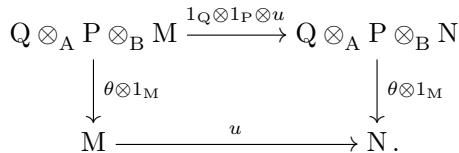
\includegraphics[keepaspectratio]{images/part001_2598f5b2.jpg}}

定理 1. —— 设 A 与 B 是 k-代数，P 是一个 \((A,B)_{k}\)-双模。把 \((B,A)_{k}\)-双模 \(\operatorname{Hom}_{\mathrm{A}}(\mathrm{P},\mathrm{A}_{s})\) 记作 \(P^{*}\)。下列性质等价：

\begin{enumerate}
\def\labelenumi{(\roman{enumi})}
\item
  \((\mathrm{A},\mathrm{B})_k\)-双模 P 是可逆的。
\item
  A-模 P 是投射的、有限生成的且是生成模，且映射 \(b \mapsto b_{P}\)（从 B 到 \(\operatorname{End}_{\mathrm{A}}(\mathrm{P})^{\circ}\)）是 k-代数同构。
\item
  右 B-模 P 是投射的、有限生成的且是生成模，且映射 \(a \mapsto a_{P}\)（从 A 到 \(\operatorname{End}_{\mathrm{B}}(\mathrm{P})\)）是 k-代数同构。若这些性质成立，则同态
\end{enumerate}

\[
\Theta : \mathrm{P} ^ {*} \otimes \mathrm{P} \to {} _ {s} \mathrm{B} _ {d} \quad \text{且} \quad \Lambda : \mathrm{P} \otimes \mathrm{P} ^ {*} \to {} _ {s} \mathrm{A} _ {d}
\]

均为同构，于是 \((\mathrm{B},\mathrm{A})_k\)-双模 \(\mathrm{P}^*\) 是 \(\mathrm{P}\) 的一个逆。

若性质 (ii) 成立，则 P 是一个可逆 \((\mathrm{A},\mathrm{B})_{k}\)-双模，其逆为 \(P^{*}\)（VIII, 第 98 页，命题 2 及第 98 页，命题 3）。这就证明了 (ii) 蕴含 (i) 以及最后一个断言。

设 \((\mathrm{A},\mathrm{B})_{k}\)-双模 P 是可逆的。那么 A-模 P 是生成模（VIII, 第 98 页，命题 3, (iii) \(\Rightarrow\) (i)）。因而它是忠实的且平衡的（VIII, 第 82 页，定理 2），于是映射 \(a \mapsto a_{p}\)（从 A 到 \(\operatorname{End}_{\mathrm{B}}(\mathrm{P})\)）是双射。

现在证明映射 \(b \mapsto b_{\mathrm{P}}\)（从 B 到 \(\mathrm{End}_{\mathrm{A}}(\mathrm{P})\)）是双射。设 Q 是一个 \((\mathrm{B},\mathrm{A})_k\)-双模，它是 P 的逆。设 \(u \in \mathrm{End}_{\mathrm{A}}(\mathrm{P})\)；则 \(1_{\mathrm{Q}} \otimes u\) 是左 B-模 \(\mathbf{Q} \otimes_{\mathrm{A}} \mathbf{P}\) 的一个自同态。由于 \((\mathrm{B},\mathrm{B})_k\)-双模 \(\mathbf{Q} \otimes_{\mathrm{A}} \mathbf{P}\) 同构于 \({}_s\mathbf{B}_d\)，存在 B 中唯一的元素 \(b\)，使得 \(1_{\mathrm{Q}} \otimes u\) 是以 \(b\) 为比的、右 B-模 \(\mathbf{Q} \otimes_{\mathrm{A}} \mathbf{P}\) 的位似。于是我们有 \(1_{\mathrm{Q}} \otimes (u - b_{\mathrm{P}}) = 0\)。从而由引理 1 得 \(u = b_{\mathrm{P}}\)；这就证明了映射 \(b \mapsto b_{\mathrm{P}}\)（从 B 到 \(\operatorname{End}_{\mathrm{A}}(\mathrm{P})\)）是双射。

于是由 VIII, 第 98 页的命题 2，A-模 P 是投射的且有限生成的。这样我们就证明了 (i) 与 (ii) 的等价性。

交换 A 与 B 的角色，即得 (i) 与 (iii) 的等价性，命题证毕。

推论 1. —— 设 A 与 B 是森田等价的 k-代数，P 是一个可逆 \((A,B)_{k}\)-双模。存在一个同构 \(\varphi\)，从 A 的中心 \(Z(A)\) 到 B 的中心，它由关系式 \(\varphi(z)_{\mathrm{P}} = z_{\mathrm{P}}\)（对每个 \(z \in Z(A)\)）确定。\((A,B)_{k}\)-双模 P 的自同构是诸位似 \(z_{P}\)，其中 z 是 \(Z(A)\) 的一个可逆元素。

给定定理 1，这由 VIII, 第 97 页的注 2 得出。

推论 2. —— 设 A 与 B 是森田等价的 k-代数，P 是一个可逆 \((\mathrm{A},\mathrm{B})_{k}\)-双模。每个与 P 互逆的 \((\mathrm{B},\mathrm{A})_{k}\)-双模都同构于 P 的对偶 \(\mathrm{P}^{*}=\mathrm{Hom}_{\mathrm{A}}(\mathrm{P},\mathrm{A})\)。更精确地说，设 Q 是一个作为 P 的逆的 \((\mathrm{B},\mathrm{A})_{k}\)-双模，\(\lambda:P\otimes_{B}Q\to_{s}A_{d}\) 是 \((\mathrm{A},\mathrm{A})_{k}\)-双模的一个同构。存在唯一的映射 \(\tau:\mathrm{Q}\to\mathrm{P}^{*}\)，它由关系式 \(\langle p,\tau(q)\rangle=\lambda(p\otimes q)\)（\(p\in P\)，\(q\in Q\)）确定，且 \(\tau\) 是 \((\mathrm{B},\mathrm{A})_{k}\)-双模的同构。

映射 \(\tau\) 的存在性与唯一性是明显的。它是 \((\mathrm{B},\mathrm{A})_{k}\)-双模的同态，并且我们有 \(\lambda=\Lambda\circ(1_{\mathrm{P}}\otimes\tau)\)。由于 \(\lambda\) 与 \(\Lambda\) 都是 \((\mathrm{A},\mathrm{A})_{k}\)-双模的同构（VIII, 第 101 页，定理 1），\(1_{P}\otimes\tau\) 亦是。由引理 1，映射 \(\tau\) 是双射。

注. —— 在该推论的假设下，设 q 是 Q 的一个元素，使得 \(\lambda(p \otimes q) = 0\)（对每个 \(p \in P\)）。那么我们有 \(\tau(q) = 0\)，即 q = 0。同样，若 p 是 P 的一个元素，使得 \(\lambda(p \otimes q) = 0\)（对每个 \(q \in Q\)），则 p = 0。

例. —— 1) 设 B 是一个 \(k\)-代数，\(n\) 是一个 \(\geqslant 1\) 的整数，A 是 \(k\)-代数 \(\mathbf{M}_n(\mathrm{B})\)。右 B-模 \(\mathrm{P} = \mathrm{B}_d^n\) 是投射的、有限生成的且是生成模，并且 A 可以等同于 P 的自同态代数（II, §10, No.~7, 第 349 页）。由定理 1，\((\mathrm{A},\mathrm{B})_k\)-双模 P 是可逆的。于是代数 B 与 \(\mathbf{M}_n(\mathrm{B})\) 是森田等价的。

\begin{enumerate}
\def\labelenumi{\arabic{enumi})}
\setcounter{enumi}{1}
\tightlist
\item
  *设 A 是一个交换 \(k\)-代数，P 是一个 A-模。我们把 P 视为一个两个作用律相等的 \((A, A)_k\)-双模。若 \((A, A)_k\)-双模 P 是可逆的，则 A-模 P 是有限生成的（定理 1）。由《交换代数》II, §5, No.~4, 第 114 页的定理 3，下列性质等价：
\end{enumerate}

\begin{enumerate}
\def\labelenumi{(\roman{enumi})}
\item
  \((\mathrm{A},\mathrm{A})_{k}\)-双模 P 是可逆的。
\item
  存在一个 A-模 \(\mathrm{Q}\)，使得 \(\mathrm{P} \otimes_{\mathrm{A}} \mathrm{Q}\) 同构于 \(\mathrm{A}\)。
\item
  A-模 P 是投射的、有限生成的，且秩为 1。 *
\end{enumerate}

\subsection{模的森田对应}

在本小节中，字母 A 与 B 表示森田等价的 k-代数，P 表示一个可逆 \((A,B)_{k}\)-双模。取定一个与 P 互逆的 \((B,A)_{k}\)-双模 Q 以及同构

\[
\lambda : \mathrm{P} \otimes_ {\mathrm{B}} \mathrm{Q} \rightarrow {} _ {s} \mathrm{A} _ {d} \quad \text { and } \quad \theta : \mathrm{Q} \otimes_ {\mathrm{A}} \mathrm{P} \rightarrow {} _ {s} \mathrm{B} _ {d}.
\]

对每个左 B-模 V，用 \(\theta_{V}\) 表示 B-模同态 \(\theta\otimes1_{V}:Q\otimes_{A}P\otimes_{B}V\to V\)；由于 \(\theta\) 是同构，它是同构。同样，对每个左 A-模 M，用 \(\lambda_{M}\) 表示 A-模同态 \(\lambda\otimes1_{M}:P\otimes_{B}Q\otimes_{A}M\to M\)；由于 \(\lambda\) 是同构，它是同构。

定理 2（森田）. —— a) 设 V 与 W 是左 B-模。映射 \(g \mapsto 1_{\mathrm{P}} \otimes g\) 是从 \(\operatorname{Hom}_{\mathrm{B}}(\mathrm{V}, \mathrm{W})\) 到 \(\operatorname{Hom}_{\mathrm{A}}(\mathrm{P} \otimes_{\mathrm{B}} \mathrm{V}, \mathrm{P} \otimes_{\mathrm{B}} \mathrm{W})\) 的双射。逆双射把 \(\operatorname{Hom}_{\mathrm{A}}(\mathrm{P} \otimes_{\mathrm{B}} \mathrm{V}, \mathrm{P} \otimes_{\mathrm{B}} \mathrm{W})\) 的元素 h 映为元素 \(\theta_{\mathrm{W}} \circ (1_{\mathrm{Q}} \otimes h) \circ \theta_{\mathrm{V}}^{-1}\)，它属于 \(\operatorname{Hom}_{\mathrm{B}}(\mathrm{V}, \mathrm{W})\)。

\begin{enumerate}
\def\labelenumi{\alph{enumi})}
\setcounter{enumi}{1}
\tightlist
\item
  每个左 A-模 M 都同构于形如 \(\mathrm{P} \otimes_{\mathrm{B}} \mathrm{V}\) 的模，其中 V 是左 B-模。
\end{enumerate}

设 V 与 W 是左 B-模。由 VIII, 第 101 页的引理 1，映射 \(\varphi : g \mapsto 1_{\mathrm{P}} \otimes g\)（从 \(\mathrm{Hom}_{\mathrm{B}}(\mathrm{V}, \mathrm{W})\) 到 \(\mathrm{Hom}_{\mathrm{A}}(\mathrm{P} \otimes_{\mathrm{B}} \mathrm{V}, \mathrm{P} \otimes_{\mathrm{B}} \mathrm{W})\)）是单射。交换 P 与 Q（以及 A 与 B）的角色，可见映射 \(\psi : h \mapsto 1_{\mathrm{Q}} \otimes h\)（从 \(\mathrm{Hom}_{\mathrm{A}}(\mathrm{P} \otimes_{\mathrm{B}} \mathrm{V}, \mathrm{P} \otimes_{\mathrm{B}} \mathrm{W})\) 到 \(\mathrm{Hom}_{\mathrm{A}}(\mathrm{Q} \otimes_{\mathrm{A}} \mathrm{P} \otimes_{\mathrm{B}} \mathrm{V}, \mathrm{Q} \otimes_{\mathrm{A}} \mathrm{P} \otimes_{\mathrm{B}} \mathrm{W})\)）也是单射。而复合 \(\psi \circ \varphi\) 是映射 \(g \mapsto \theta_{\mathrm{W}}^{-1} \circ g \circ \theta_{\mathrm{V}}\)。它是双射，因而 \(\psi\) 也是。于是 \(\varphi\) 是双射，其逆是映射 \(h \mapsto \theta_{\mathrm{W}} \circ (1_{\mathrm{Q}} \otimes h) \circ \theta_{\mathrm{V}}^{-1}\)。

断言 b) 由 \(\lambda_{\mathrm{M}}\) 是从 \(\mathrm{P} \otimes_{\mathrm{B}} \otimes_{\mathrm{A}} \otimes_{\mathrm{M}}\) 到 \(\mathrm{M}\) 的同构这一事实得出。

设 V 是一个左 B-模，W 是 V 的一个子模。由于 B-模 P 是投射的（VIII, 第 101 页，定理 1），从 \(P \otimes_{B} W\) 到 \(P \otimes_{B} V\) 的典范映射是单射。我们借此映射把 \(P \otimes_{B} W\) 与它在 \(P \otimes_{B} V\) 中的像等同起来。当 P 与 B 分别换成 Q 与 A 时，我们采用类似的约定。

命题 5. —— 设 V 是一个左 B-模。映射 \(W \mapsto P \otimes_{B} W\) 是从 V 的 B-子模之集（按包含关系排序）到 \(P \otimes_{B} V\) 的 A-子模之集（按包含关系排序）的同构。逆同构把 \(P \otimes_{B} V\) 的 A-子模 N 映为 \(\theta_{V}\) 作用下 B-子模 \(Q \otimes_{A} N\)（\(Q \otimes_{A} P \otimes_{B} V\) 的子模）的像。

用 \(D_{\mathrm{B}}(\mathrm{V})\) 表示 V 的按包含关系排序的 B-子模之集，并同样地定义集合 \(D_{\mathrm{A}}(\mathrm{P}\otimes_{\mathrm{B}}\mathrm{V})\) 与 \(D_{\mathrm{B}}(\mathrm{Q}\otimes_{\mathrm{A}}\mathrm{P}\otimes_{\mathrm{B}}\mathrm{V})\)。设 \(\varphi:D_{\mathrm{B}}(\mathrm{V})\to D_{\mathrm{A}}(\mathrm{P}\otimes_{\mathrm{B}}\mathrm{V})\) 是映射 \(W\mapsto P\otimes_{B}W\)，\(\psi\) 是从 \(D_{\mathrm{A}}(\mathrm{P}\otimes_{\mathrm{B}}\mathrm{V})\) 到 \(D_{\mathrm{B}}(\mathrm{Q}\otimes_{\mathrm{A}}\mathrm{P}\otimes_{\mathrm{B}}\mathrm{V})\) 的映射，由 \(N\mapsto Q\otimes_{A}N\) 给出。它们都是递增映射，且复合 \(\psi\circ\varphi\) 是映射 \(W\mapsto\theta_{\mathrm{V}}^{-1}(\mathrm{W})\)，后者是双射。于是 \(\varphi\) 是单射，而 \(\psi\) 是满射。把 B 换成 A、V 换成 \(P\otimes_{B}V\)，即见 \(\psi\) 也是单射。从而 \(\varphi\) 与 \(\psi\) 都是双射，且 \(\varphi\) 的逆映射正是命题中所描述的那个。

例. —— 1) 把 VIII, 第 104 页的命题 5 应用于特殊情形 \(\mathrm{V} = \mathrm{B}_s\)。

\begin{enumerate}
\def\labelenumi{\alph{enumi})}
\item
  映射 \(J \mapsto PJ\) 是从 B 的左理想的有序集 \(\mathrm{D}(\mathrm{B}_{s})\) 到 P 的 A-子模的有序集 \(\mathrm{D}(\mathrm{P})\) 的同构。逆映射把 P 的 A-子模 M 映为 B 的左理想 \(\mathrm{J}(\mathrm{M})\)，它由 B 中使 M 包含 Pb 的元素 b 组成。
\item
  映射 \(K \mapsto KP\) 是从 A 的右理想的有序集 \(\mathrm{D}(A_{d})\) 到 P 的 B-子模的有序集 \(\mathrm{D}(P)\) 的同构。逆映射把 P 的 B-子模 V 映为 A 的右理想 \(\mathrm{K}(V)\)，它由 A 中使 V 包含 aP 的元素 a 组成。
\end{enumerate}

事实上，A-模 \(P \otimes_{B} B_{s}\) 可以典范地等同于 P。若 J 是 B 的一个左理想，则 \(P \otimes_{B} J\) 在 \(P \otimes_{B} B_{s}\) 中的典范像在此等同下对应于 PJ。于是映射 \(J \mapsto PJ\) 是从 \(D(B_{s})\) 到 \(D(P)\) 的有序集同构。设 \(J \in D(B_{s})\)。用 \(J'\) 表示 B 中使 PJ 包含 Pb 的元素 b 之集。它是 B 的包含 J 的左理想，并且我们有 \(PJ' \subset PJ\)。由于映射 \(J \mapsto PJ\) 是有序集的同构，必然有 \(PJ' = PJ\) 及 \(J = J'\)。这就证明了 a)。

断言 b) 由把断言 a) 应用于可逆 \((\mathrm{B}^{\circ},\mathrm{A}^{\circ})_{k}\)-双模 P 得出。

注意，环 A 是体当且仅当 B-模 P 是单模。

\begin{enumerate}
\def\labelenumi{\arabic{enumi})}
\setcounter{enumi}{1}
\tightlist
\item
  用 \(\mathcal{B}_{\mathrm{A}}\)、\(\mathcal{B}_{\mathrm{B}}\) 与 \(\mathcal{B}_{\mathrm{P}}\) 分别表示 A 的双边理想之集、B 的双边理想之集与 P 的 \((\mathrm{A},\mathrm{B})_k\)-子双模之集。
\end{enumerate}

\begin{enumerate}
\def\labelenumi{\alph{enumi})}
\item
  映射 \(\mathfrak{b} \mapsto \mathrm{P}\mathfrak{b}\) 是从 \(\mathcal{B}_{\mathrm{B}}\) 到 \(\mathcal{B}_{\mathrm{P}}\) 的有序集同构；逆同构把一个 \((\mathrm{A},\mathrm{B})_k\)-子双模 \(\mathrm{P}'\)（\(\mathrm{P}\) 的）映为 \(\mathrm{B}\) 的由元素 \(b\)（使得 \(\mathrm{P}b \subset \mathrm{P}'\)）组成的双边理想。
\item
  映射 \(a \mapsto aP\) 是从 \(B_{A}\) 到 \(B_{P}\) 的有序集同构；逆同构把 P 的 \((A, B)_{k}\)-子双模 \(P'\) 映为 A 的由使 \(aP \subset P'\) 的元素 a 组成的双边理想。
\end{enumerate}

事实上，设 J 是 B 的一个左理想，且 \(P' = PJ\)。那么 \(P'\) 是 P 的 A-子模，并且由例 1，理想 J 由 B 中使 \(Pb \subset P'\) 的元素 b 组成。此外，\(P'\) 是 P 的 \((A, B)_{k}\)-子双模当且仅当 J 是 B 的双边理想。于是 a) 由同前所引得出。

断言 b) 由把断言 a) 应用于可逆 \((\mathrm{B}^{\circ}, \mathrm{A}^{\circ})_{k}\)-双模 P 得出。

命题 6. —— 用 \(\mathcal{B}_{\mathrm{A}}\) 与 \(\mathcal{B}_{\mathrm{B}}\) 表示 A 的双边理想之集与 B 的双边理想之集。

\begin{enumerate}
\def\labelenumi{\alph{enumi})}
\item
  存在一个有序集同构 \(f\)，从 \(\mathcal{B}_{\mathrm{A}}\) 到 \(\mathcal{B}_{\mathrm{B}}\)，它由下列性质确定：若 \(\mathfrak{a}\) 是 \(\mathrm{A}\) 的双边理想，\(\mathfrak{b}\) 是 \(\mathrm{B}\) 的双边理想，则关系 \(f(\mathfrak{a}) = \mathfrak{b}\) 等价于 \(\mathfrak{a}\mathrm{P} = \mathrm{P}\mathfrak{b}\)。
\item
  设环 A 是交换的，从而 A 可等同于 B 的中心（VIII, 第 102 页，推论 1）。同构 \(f: \mathcal{B}_{\mathrm{A}} \to \mathcal{B}_{\mathrm{B}}\) 把 A 的理想 \(\mathfrak{a}\) 映为 B 的双边理想 \(\mathrm{Ba}\)，并且我们有 \(\mathfrak{a} = \mathrm{A} \cap \mathrm{Ba}\)。
\end{enumerate}

断言 a) 由例 2 得出。

现在设 A 是交换的，并把 A 等同于 B 的中心。设 a 是 A 的一个理想。那么 Ba 是 B 的双边理想；我们有 PBa = aP，因此 \(f(a) = \text{Ba}\)。设 \(a'\) 是 A 的理想 \(A \cap Ba\)；它含于 Ba 且包含 a，故 \(Ba'\) 等于 Ba。由于 f 是双射，由此得 \(a' = a\)。

例. —— 3) 设 V 是一个左 B-模。那么上面给出的对应把 B-模 V 的零化理想映为 A-模 \(P \otimes_{B} V\) 的零化理想。事实上，用 a 表示 A-模 \(P \otimes_{B} V\) 的零化理想，用 b 表示 B-模 V 的零化理想。设 W 是 P 的 \((A, B)_{k}\)-子双模，它由使对 V 的每个元素 v 都有 \(p \otimes v = 0\) 的元素组成。我们有包含关系 \(Pb \subset W\)；反之，对每个 \(p \in W\) 与 \(q \in Q\)，我们有 \(\theta(q \otimes p)\) 属于 b。于是，\(D(B_s)\) 的元素 b 对应于 D(P) 的元素 W。同样，\(a \in D(A_d)\) 对应于 W。

\begin{enumerate}
\def\labelenumi{\arabic{enumi})}
\setcounter{enumi}{3}
\tightlist
\item
  对 A 的每个双边理想 \(\mathfrak{a}\)，把 \(\mathbf{M}_n(\mathrm{A})\) 中由系数属于 \(\mathfrak{a}\) 的矩阵组成的子集记作 \(\mathbf{M}_n(\mathfrak{a})\)。它是 \(\mathbf{M}_n(\mathrm{A})\) 的双边理想。我们有 \(\mathbf{M}_n(\mathfrak{a})\mathrm{A}^n = \mathfrak{a}^n = \mathrm{A}^n\mathfrak{a}\)。由命题 6 推出，\(\mathbf{M}_n(\mathrm{A})\) 的每个双边理想都形如 \(\mathbf{M}_n(\mathfrak{a})\)，其中 \(\mathfrak{a}\) 是 A 的双边理想。
\end{enumerate}

注. —— 我们保留上面的假设与记号，并设 \((\mathrm{B},\mathrm{A})_{k}\)-双模 Q 是 A-模 P 的对偶 \(P^{*}\)，同构 \(\lambda\) 与 \(\theta\) 是典范映射 \(\Lambda:P\otimes_{B}P^{*}\to_{s}A_{d}\) 与 \(\Theta:P^{*}\otimes_{A}P\to_{s}B_{d}\)（VIII, 第 101 页，定理 1）。由于 A-模 P 是投射的且有限生成的，对每个 A-模 M 我们有一个典范同构 \(\vartheta_{M}:P^{*}\otimes_{A}M\to\operatorname{Hom}_{A}(P,M)\)（II, §4, No.~2, 第 271 页，推论）。我们把将构造 \(M\mapsto Q\otimes_{A}M\) 换成构造 \(M\mapsto\operatorname{Hom}_{A}(P,M)\) 后对第 3、4 小节结果的改述留给读者。

\subsection{子模的有序集}

在本小节中，A 与 B 是 k-代数，M 是一个左 A-模，V 是一个左 B-模。我们用 \(\mathrm{D}(\mathrm{M})\)（相应地，\(\mathrm{D}(\mathrm{V})\)）表示 M（相应地，V）的按包含关系排序的子模之集。我们设给定了有序集的同构 \(\varphi : \mathrm{D}(\mathrm{V}) \to \mathrm{D}(\mathrm{M})\)。

由森田定理（VIII, 第 103 页，定理 2），在下列情形我们得到这样一个同构：P 是一个可逆 \((\mathrm{A},\mathrm{B})_k\)-双模，M 是 A-模 \(\mathrm{P} \otimes_{\mathrm{B}} \mathrm{V}\)，并且对 V 的每个子模 W，\(\varphi(\mathrm{W})\) 是 \(\mathrm{P} \otimes_{\mathrm{B}} \mathrm{W}\) 在 M 中的典范像。

模 M 的某些性质，或其子模的某些性质，可以用有序集 D(M) 来表达：它们列于表 I 与表 II 中。

模 M 是子模族 \((\mathrm{M}_{i})_{i\in\mathrm{I}}\) 的直和当且仅当我们有 \(M=\sum_{i\in I}M_{i}\) 与 \(M_{i}\cap\sum_{j\neq i}M_{j}=0\)（对每个 \(i\in I\)）。这一注记以及对表 I 的考察给出下面的结果。

命题 7. —— a) 我们有 \(\varphi(0)=0\) 及 \(\varphi(V)=M\)。

\begin{enumerate}
\def\labelenumi{\alph{enumi})}
\setcounter{enumi}{1}
\tightlist
\item
  设 \((\mathrm{V}_i)_{i\in \mathrm{I}}\) 是 V 的一个子模族。我们有
\end{enumerate}

\[
\varphi \left(\sum_ {i \in \mathrm{I}} \mathrm{V} _ {i}\right) = \sum_ {i \in \mathrm{I}} \varphi (\mathrm{V} _ {i}), \quad \varphi \left(\bigcap_ {i \in \mathrm{I}} \mathrm{V} _ {i}\right) = \bigcap_ {i \in \mathrm{I}} \varphi (\mathrm{V} _ {i}).
\]

M 的子模

有序集 D(M)

零子模

D(M) 的最小元

子模 M

D(M) 的最大元

\(\bigcap_{i\in I} M_i\)

下确界 \(\inf_{i\in I} M_i\)

\(\sum_{i\in I} M_i\)

上确界 \(\sup_{i\in I} M_i\)

互补子模

\(\inf(M', M'') = 0, \sup(M', M'') = M\)

M 的单子模

D(M) --- \{0\} 的极小元

M 的极大子模

D(M) --- \{M\} 的极大元

M 的底座 \(\mathscr{S}(M)\)

D(M) --- \{0\} 的极小元之集在 D(M) 中的上确界

\emph{M 的根 \(\Re(M)\)}（VIII, 第 151 页）

D(M) --- \{M\} 的极大元之集在 D(M) 中的下确界

模 M 的性质

D(M) 的性质

M 是诺特模。

有序集 D(M) 是诺特的（《集合论》III, §6, No.~5, 第 190 页）。

M 是阿廷模。

按 ⊃ 排序的集合 D(M) 是诺特的。

M 是不可分解的。

我们有 M ≠ 0，并且不存在 D(M) 的两个非零元素 M\textquotesingle{} 与 M\textquotesingle\textquotesingle{} 满足 inf(M\textquotesingle, M\textquotesingle\textquotesingle) = 0, sup(M\textquotesingle, M\textquotesingle\textquotesingle) = M。

M 是有限生成的。

对 D(M) 中每个以 M 为上界的族 (Mi) i∈I，存在 I 的有限子集 J，使 M = supj∈I Mj。

M 是单模。

Card(D(M)) = 2。

M 是半单的。

M 是 D(M) = \{0\} 的极小元之集在 D(M) 中的上确界。

表 II.

\begin{enumerate}
\def\labelenumi{\alph{enumi})}
\setcounter{enumi}{2}
\tightlist
\item
  B-模 V 是子模族 \((\mathrm{V}_{i})_{i\in\mathrm{I}}\) 的直和当且仅当 M 是子模族 \((\varphi(\mathrm{V}_{i}))_{i\in\mathrm{I}}\) 的直和。
\end{enumerate}

设 \(V'\) 与 \(V''\) 是 \(V\) 的子模，使得 \(V'\) 含于 \(V''\)；令 \(M' = \varphi(V')\)，\(M'' = \varphi(V'')\)，于是 \(M''\) 包含 \(M'\)。用 \([V', V'']\) 表示 \(D(V)\) 中由子模 \(W\)（属于 \(V\)，满足 \(V' \subset W \subset V''\)）组成的区间，并同样地定义区间 \([M', M'']\)（在 \(D(M)\) 中）。映射 \(W \mapsto W/V'\) 是从 \([V', V'']\) 到 \(D(V''/V')\) 的有序集同构；我们同样地定义从 \([M', M'']\) 到 \(D(M''/M')\) 的有序集同构。由于 \(\varphi\) 把区间 \([V', V'']\) 映到 \([M', M'']\)，它定义了一个有序集同构 \(\varphi\)，从 \(D(V''/V')\) 到 \(D(M''/M')\)。我们由此以及表 I 与表 II 推出下面的命题。

命题 8. —— a) 设 V' 与 V'\,' 是 V 的子模，使得 V'\,' 包含 V'。B-模 V'\,'/V' 是单模当且仅当 A-模 \(\varphi(\mathrm{V}^{\prime\prime})/\varphi(\mathrm{V}^{\prime})\) 是单模。

\begin{enumerate}
\def\labelenumi{\alph{enumi})}
\setcounter{enumi}{1}
\item
  若 \(V'\) 是 V 的单子模、极大子模或直因子，则 \(\varphi(V')\) 相应地是 M 的单子模、极大子模或直因子。
\item
  同构 \(\varphi\) 把底座 \(\mathcal{S}(\mathrm{V})\)（\(\mathrm{V}\) 的）变为底座 \(\mathcal{S}(\mathrm{M})\)（\(\mathrm{M}^*\) 的），把根（VIII, 第 151 页，定义 1）\(\Re (\mathrm{V})\)（\(\mathrm{V}\) 的）变为根 \(\Re (\mathrm{M})\)（\(\mathrm{M}_{*}\) 的）
\item
  设 \((\mathrm{V}_{i})_{0\leqslant i\leqslant n}\) 是 V 的子模的一个有限序列。它是 V 的若尔当–赫尔德列当且仅当 \((\varphi(\mathrm{V}_{i})_{0\leqslant i\leqslant n})\) 是 M 的若尔当–赫尔德列。
\end{enumerate}

引理 2. —— 设 H 与 H' 是 V 的子模，满足 \(H \cap H' = 0\)。B-模 H 与 H' 同构当且仅当 A-模 \(\varphi(\mathrm{H})\) 与 \(\varphi(\mathrm{H}')\) 同构。

我们把 \(H+H'\) 等同于乘积 \(H \times H'\)。从 H 到 \(H'\) 的一个同构的图像是 V 的一个子模 \(H''\)，它满足

\[
\mathrm{H} \cap \mathrm{H} ^ {\prime \prime} = \mathrm{H} ^ {\prime} \cap \mathrm{H} ^ {\prime \prime} = 0, \quad \mathrm{H} + \mathrm{H} ^ {\prime} = \mathrm{H} + \mathrm{H} ^ {\prime \prime} = \mathrm{H} ^ {\prime} + \mathrm{H} ^ {\prime \prime};\tag{17}
\]

反之，每个具有这些性质的子模是从 H 到 \(H'\) 的一个同构的图像。由命题 7，关系 \(H \cap H' = 0\) 等价于 \(\varphi(\mathrm{H}) \cap \varphi(\mathrm{H}') = 0\)，而关系式 (17) 等价于关系式

\[
\varphi (\mathrm{H}) \cap \varphi (\mathrm{H} ^ {\prime \prime}) = \varphi (\mathrm{H} ^ {\prime}) \cap \varphi (\mathrm{H} ^ {\prime \prime}) = 0,
\]

\[
\varphi (\mathrm{H}) + \varphi (\mathrm{H} ^ {\prime}) = \varphi (\mathrm{H}) + \varphi (\mathrm{H} ^ {\prime \prime}) = \varphi (\mathrm{H} ^ {\prime}) + \varphi (\mathrm{H} ^ {\prime \prime});
\]

引理由此得出。

命题 9. —— 设 S 是 V 的一个单子模，T 是 M 的单子模 \(\varphi(\mathrm{S})\)。若用 \(V_{S}\) 表示 V 的 S 型同型分量，用 \(M_{T}\) 表示 M 的 T 型同型分量，则我们有 \(\varphi(V_{\mathrm{S}})=M_{\mathrm{T}}\)。

V 的每个异于 S 的单子模 \(S'\) 满足 \(S' \cap S = 0\)。因此它同构于 S 当且仅当 \(\varphi(S')\) 同构于 T（引理 2）。而 \(V_{S}\) 是 V 的同构于 S 的单子模之和，\(M_{T}\) 是 M 的同构于 T 的单子模之和。于是命题 9 由命题 7 与命题 8 立即得出。

命题 10. —— a) B-模 V 是阿廷的（相应地，诺特的、不可分解的、单的、有限生成的）当且仅当 M 亦然。

\begin{enumerate}
\def\labelenumi{\alph{enumi})}
\setcounter{enumi}{1}
\item
  B-模 V 具有有限长度当且仅当 A-模 M 具有有限长度，且此时我们有 \(\mathrm{long}_{\mathrm{B}}(\mathrm{V}) = \mathrm{long}_{\mathrm{A}}(\mathrm{M})\)。
\item
  B-模 V 是半单的（相应地，同型的）当且仅当 A-模 M 是半单的（相应地，同型的）。若情形如此，则我们有 \(\text{long}_{\text{B}}(\text{V}) = \text{long}_{\text{A}}(\text{M})\)。
\end{enumerate}

断言 a) 由表 II 中所列的第二条性质得出。

断言 b) 由命题 8, d) 得出。

模 V 是半单的当且仅当它等于其底座 \(\mathcal{S}(V)\)；它是同型的当且仅当存在 V 的一个单子模 S，使得 \(V = V_{S}\)。于是断言 c) 由命题 7, c)、8, c) 与 9（VIII, 第 106 页与第 109 页）得出。

\subsection{森田对应下保持的其他性质}

设 A 与 B 是森田等价的 k-代数，P 是一个可逆 \((A,B)_{k}\)-双模。

命题 11. —— 设

\[
\mathrm{V} ^ {\prime} \xrightarrow {f} \mathrm{V} \xrightarrow {g} \mathrm{V} ^ {\prime \prime}\tag{ε}
\]

是一个由 B-模与 B-线性映射组成的图，并设

\[
(\mathrm{P} \otimes \mathcal {E})
\]

\[
\mathrm{P} \otimes_ {\mathrm{B}} \mathrm{V} ^ {\prime} \xrightarrow {1 _ {\mathrm{P}} \otimes f} \mathrm{P} \otimes_ {\mathrm{B}} \mathrm{V} \xrightarrow {1 _ {\mathrm{P}} \otimes g} \mathrm{P} \otimes_ {\mathrm{B}} \mathrm{V} ^ {\prime \prime}
\]

是相应的 A-模的图。那么 \((\mathcal{E})\) 是正合列当且仅当 \((\mathrm{P} \otimes \mathcal{E})\) 是正合列。

设序列 \((\mathcal{E})\) 是正合的。由于右 B-模 P 是投射的，序列 \((P \otimes \mathcal{E})\) 是正合的（II, §3, No.~6, 第 251 页，命题 5 及 II, §3, No.~7, 第 257 页，推论 6）。

反之，设序列 \((\mathrm{P} \otimes \mathcal{E})\) 是正合的。设 Q 是一个 \((\mathrm{B}, \mathrm{A})_{k}\)-双模，它是 P 的逆，并设 \(\theta : Q \otimes_{A} P \to {}_{s} B_{d}\) 是一个同构。考虑交换图

\[
\begin{array}{c} \mathrm{Q} \otimes_ {\mathrm{A}} \mathrm{P} \otimes_ {\mathrm{B}} \mathrm{V} ^ {\prime} \xrightarrow {1 _ {\mathrm{Q}} \otimes 1 _ {\mathrm{P}} \otimes f} \mathrm{Q} \otimes_ {\mathrm{A}} \mathrm{P} \otimes_ {\mathrm{B}} \mathrm{V} \xrightarrow {1 _ {\mathrm{Q}} \otimes 1 _ {\mathrm{P}} \otimes g} \mathrm{Q} \otimes_ {\mathrm{A}} \mathrm{P} \otimes_ {\mathrm{B}} \mathrm{V} ^ {\prime \prime} \\ \theta \otimes 1 _ {\mathrm{V} ^ {\prime}} \Biggl \downarrow \\ \mathrm{V} ^ {\prime} \xrightarrow {f} \mathrm{V} \xrightarrow {g} \mathrm{V} ^ {\prime \prime}. \end{array}
\]

由于 Q 是投射 A-模且序列 \((\mathrm{P} \otimes \mathcal{E})\) 是正合的，此图的第一行是一个正合列。由于诸竖直箭头都是同构，第二行也是正合的。

推论. —— 设 \(f: V \rightarrow W\) 是一个 B-线性映射。那么 f 是单射（相应地，满射）当且仅当 \(1_{P} \otimes f\) 是。

命题 12. —— 设 V 是一个左 B-模。B-模 V 是投射的（相应地，是生成模、忠实的、*内射的、有限表现的*）当且仅当 A-模 P ⊗\_B V 亦然。

\begin{enumerate}
\def\labelenumi{\alph{enumi})}
\item
  设 V 是投射的。存在一个集合 I，使 V 同构于 \(\mathrm{B}_{s}^{(\mathrm{I})}\) 的一个直因子子模。于是 A-模 \(P \otimes_{B} V\) 同构于 \(\mathrm{P}^{(\mathrm{I})}\) 的一个直因子子模；由于 P 是投射 A-模，\(P \otimes_{B} V\) 亦然。
\item
  设 B-模 V 是生成模。设 M 是一个 A-模。存在一个 B-模 W，使 M 同构于 \(P \otimes_{B} W\)。由 VIII, 第 80 页的定理 1，存在一个集合 I 与一个满射 \(\varphi : V^{(I)} \to W\)。由该推论，映射 \(1_{P} \otimes \varphi\)（从 \(P \otimes (V^{(I)})\) 到 \(P \otimes_{A} W\)）是满射，这给出一个满射 \((P \otimes V)^{(I)} \to M\)。由 VIII, 第 80 页的定理 1，\(P \otimes V\) 是生成 A-模。
\item
  B-模 V 是忠实的当且仅当它的零化理想约化为 0。于是断言 c) 由 VIII, 第 105 页的例 3 得出。
\end{enumerate}

*d) 设 V 是内射的。由 VIII, 第 106 页的注，A-模 \(\mathrm{P} \otimes_{\mathrm{B}} \mathrm{V}\) 同构于 \(\mathrm{Hom}_{\mathrm{B}}(\mathrm{Q}, \mathrm{V})\)，其中 Q 是一个与 A 互逆的 \((\mathrm{B}, \mathrm{A})_k\)-双模。由于 A-模 Q 是投射的，因而是平坦的（X, §1, n° 3, 第 9 页，例 1），由 X, §1, n° 8, 第 18 页，命题 11，A-模 \(\mathrm{Hom}_{\mathrm{B}}(\mathrm{Q}, \mathrm{V})\) 是内射的。

\begin{enumerate}
\def\labelenumi{\alph{enumi})}
\setcounter{enumi}{4}
\item
  设 V 有一个有限表现 \(L_{1} \to L_{0} \to V \to 0\)（X, §1, n° 4, 第 10 页）。用 P 作张量积，我们导出 A-模的一个正合列 \(N_{1}^{\prime} \xrightarrow{u} N_{0}^{\prime} \to P \otimes_{B} V \to 0\)，其中 \(N_{1}^{\prime}\) 与 \(N_{0}^{\prime}\) 是投射的且有限生成的（命题 11 与 a)）。设 \(N_{0}^{\prime\prime}\) 是一个有限生成 A-模，使得模 \(N_{0} = N_{0}^{\prime} \oplus N_{0}^{\prime\prime}\) 是自由的且有限生成的，并设 \(u^{\prime}: N_{1}^{\prime} \oplus N_{0}^{\prime\prime} \to N_{0}\) 是同态 \((u, 1_{N_{0}^{\prime\prime}})\)；于是 \(P \otimes_{B} V\) 可以等同于 \(u^{\prime}\) 的余核。设 \(N_{1}\) 是一个有限生成的自由 A-模，\(p: N_{1} \to N_{1}^{\prime} \oplus N_{0}^{\prime\prime}\) 是一个满射同态；序列 \(N_{1} \xrightarrow{u^{\prime} \circ p} N_{0} \to P \otimes_{B} V \to 0\) 是 A-模 \(P \otimes_{B} V_*\) 的一个有限表现
\item
  设 A-模 \(P \otimes_{B} V\) 是投射的（相应地，是生成模、忠实的、*内射的、有限表现的*）。把上面的结果应用于（交换 A 与 B 以及 P 与 Q 的角色），可见 B-模 \(Q \otimes_{A} P \otimes_{B} V\) 也具有这一性质。于是对同构于它的 B-模 V 同样如此。
\end{enumerate}

推论. —— 环 A 是左阿廷的（相应地，左诺特的）当且仅当环 B 亦然。

由于 B 的左理想的有序集与 P 的 A-子模之集之间的同构，环 B 是左阿廷的（相应地，左诺特的）当且仅当 A-模 P 是阿廷的（相应地，诺特的）。而由 VIII, 第 101 页的定理 1，A-模 P 是生成模且有限生成；特别地，\(A_{s}\) 同构于 \(P^{n}\) 的一个直因子（对一个整数 \(n \geqslant 1\)）。因此，P 是阿廷的（相应地，诺特的）当且仅当 A 是左阿廷的（相应地，左诺特的）。

\subsection{代数的森田等价}

命题 13. —— a) 若两个 k-代数是森田等价的，则它们的中心是同构的 k-代数。

\begin{enumerate}
\def\labelenumi{\alph{enumi})}
\setcounter{enumi}{1}
\item
  两个交换 \(k\)-代数森田等价当且仅当它们同构。
\item
  两个都是体的 k-代数森田等价当且仅当它们同构。
\item
  对 \(i = 1,2\)，设 \(\mathrm{A}_i\) 与 \(\mathrm{B}_i\) 是森田等价的 \(k\)-代数，\(\mathrm{P}_i\) 是一个可逆 \((\mathrm{A}_i,\mathrm{B}_i)_k\)-双模。令 \(\mathrm{A} = \mathrm{A}_1\otimes_k\mathrm{A}_2\)，\(\mathrm{B} = \mathrm{B}_1\otimes_k\mathrm{B}_2\)，\(\mathrm{P} = \mathrm{P}_1 \otimes_k \mathrm{P}_2\)。\(k\)-代数 A 与 B 是森田等价的，且 P 是一个可逆 \((\mathrm{A}, \mathrm{B})_k\)-双模。
\item
  若 A 与 B 是森田等价的 \(k\)-代数，且 \(k'\) 是一个交换 \(k\)-代数，则 \(k'\)-代数 \(\mathrm{A}_{(k')}\) 与 \(\mathrm{B}_{(k')}\) 是森田等价的。
\end{enumerate}

断言 a) 由 VIII, 第 102 页的推论 1 得出，并蕴含 b)。

设 \(\mathrm{K}\) 与 \(\mathrm{L}\) 是都是体的 \(k\)-代数，\(\mathrm{P}\) 是一个可逆 \((\mathrm{K},\mathrm{L})_k\)-双模。右 \(\mathrm{L}\)-向量空间 \(\mathrm{P}\) 是一个单模（VIII, 第 104 页），因而是 1 维的，于是 \(k\)-代数 \(\operatorname{End}_{\mathrm{L}}(\mathrm{P})\) 与 \(\mathrm{L}\) 同构。由 VIII, 第 101 页的定理 1，映射 \(a\mapsto a_{\mathrm{P}}\)（从 \(\mathrm{K}\) 到 \(\operatorname{End}_{\mathrm{L}}(\mathrm{P})\)）是一个同构。因此，体 \(\mathrm{K}\) 与 \(\mathrm{L}\) 在 \(k\) 上同构；断言 c) 得证。

在 d) 的假设下，设 \(Q_{i}\)（i = 1, 2）是一个 \((\mathrm{B}_{i}, \mathrm{A}_{i})_{k}\)-双模，与 \(P_{i}\) 互逆。用 Q 表示 \((\mathrm{B}, \mathrm{A})_{k}\)-双模 \(Q_{1} \otimes_{k} Q_{2}\)。考虑典范 k-线性同构 \((\mathrm{P}_{1} \otimes_{k} \mathrm{P}_{2}) \otimes_{k} (\mathrm{Q}_{1} \otimes_{k} \mathrm{Q}_{2}) \to (\mathrm{P}_{1} \otimes_{k} \mathrm{Q}_{1}) \otimes_{k} (\mathrm{P}_{2} \otimes_{k} \mathrm{Q}_{2})\)；在过渡到商时，它定义一个态射

\[
\left(\mathrm{P} _ {1} \otimes_ {k} \mathrm{P} _ {2}\right) \otimes_ {\mathrm{B}} \left(\mathrm{Q} _ {1} \otimes_ {k} \mathrm{Q} _ {2}\right)\rightarrow \left(\mathrm{P} _ {1} \otimes_ {\mathrm{B} _ {1}} \mathrm{Q} _ {1}\right) \otimes_ {k} \left(\mathrm{P} _ {2} \otimes_ {\mathrm{B} _ {2}} \mathrm{Q} _ {2}\right)
\]

它是 (A,A)-线性的。反之，逆同构 \((\mathrm{P}_{1}\otimes_{k}\mathrm{Q}_{1})\otimes_{k}(\mathrm{P}_{2}\otimes_{k}\mathrm{Q}_{2})\to(\mathrm{P}_{1}\otimes_{k}\mathrm{P}_{2})\otimes_{k}(\mathrm{Q}_{1}\otimes_{k}\mathrm{Q}_{2})\) 定义一个 (A,A)-线性态射 \((\mathrm{P}_{1}\otimes_{\mathrm{B}_{1}}\mathrm{Q}_{1})\otimes_{k}(\mathrm{P}_{2}\otimes_{\mathrm{B}_{2}}\mathrm{Q}_{2})\to(\mathrm{P}_{1}\otimes_{k}\mathrm{P}_{2})\otimes_{\mathrm{B}}(\mathrm{Q}_{1}\otimes_{k}\mathrm{Q}_{2})\)。这两个态射互为逆映射，从而都是同构。由于 \((\mathrm{A}_{i},\mathrm{A}_{i})\)-双模 \(P_{i}\otimes_{B_{i}}Q_{i}\) 同构于 \(A_{i}\)，我们得到一个 (A,A)-线性同构 \(P\otimes_{B}Q\to A\)。我们同样得到一个 (B,B)-线性同构 \(Q\otimes_{A}P\to B\)，这就完成了 d) 的证明。

在 e) 的假设下，设 P 是一个可逆 \((\mathrm{A},\mathrm{B})_{k}\)-双模；则 \(\mathrm{P}_{(k^{\prime})}\) 是一个可逆 \((\mathrm{A}_{(k^{\prime})},\mathrm{B}_{(k^{\prime})})_{k^{\prime}}\)-双模。

设 A 是一个 k-代数，e 是 A 中的一个幂等元。集合 eAe 赋以由 A 的加法、乘法与 k 的作用所诱导的运算，是一个以 e 为单位元的 k-代数。

命题 14. —— 设 A 与 B 是 k-代数。那么 A 与 B 森田等价当且仅当存在一个整数 \(n \geqslant 1\) 与一个方阵 \(e = (e_{ij})\)（在 \(\mathbf{M}_{n}(\mathbf{B})\) 中），满足下列条件：

\begin{enumerate}
\def\labelenumi{(\roman{enumi})}
\item
  我们有 \(e^2 = e\)。
\item
  由诸元素 \(e_{ij}\) 生成的 B 的双边理想等于 B。
\item
  \(k\)-代数 A 同构于 \(e\mathbf{M}_n(\mathrm{B})e\)。
\end{enumerate}

若条件 (i) 与 (ii) 满足，则 \((e\mathbf{M}_n(\mathrm{B})e,\mathrm{B})_k\)-双模 \(e\mathrm{B}_d^n\) 是可逆的。

鉴于定理 1（VIII, 第 101 页），k-代数 A 与 B 森田等价当且仅当它同构于一个投射的、有限生成的且是生成模的右 B-模的自同态代数。于是该命题由下面的引理 3 与引理 4 得出。

引理 3. —— 一个右 B-模 P 是投射的、有限生成的且是生成模，当且仅当存在一个整数 \(n \geqslant 0\) 与一个幂等元 \(e = (e_{ij})\)（在 \(\mathbf{M}_n(\mathrm{B})\) 中），具有下列性质：

\begin{enumerate}
\def\labelenumi{(\roman{enumi})}
\item
  B-模 P 同构于 \(e\mathrm{B}_d^n\)。
\item
  由诸元素 \(e_{ij}\) 生成的 B 的双边理想等于 B。
\end{enumerate}

设 P 是一个右 B-模。那么 P 是投射的且有限生成的，当且仅当它同构于一个形如 \(B_{d}^{n}\) 的 B-模（n 是一个 \(\geqslant 0\) 的整数）的直因子子模（II, §2, No.~2, 第 232 页，推论 1）。若我们把 k-代数 \(\mathbf{M}_{n}(\mathrm{B})\) 与 \(\operatorname{End}(\mathrm{B}_{d}^{n})\) 等同起来，则这就意味着存在 \(\mathbf{M}_{n}(\mathrm{B})\) 中的一个幂等元 e，使 P 同构于 \(eB_{d}^{n}\)。

B-模 P 是生成模当且仅当它的迹理想 \(\tau(\mathrm{P})\) 等于 B，即 \(\tau(e\mathrm{B}_{d}^{n})=\mathrm{B}\)（VIII, 第 80 页，定理 1）。设 \(x_{1},\ldots,x_{n}\) 是 \(B_{d}^{n}\) 中对应于矩阵 e 的各列的元素，并设 \(x_{i}^{*}\)（对 \(1\leqslant i\leqslant n\)）是线性形式 \((b_{1},\ldots,b_{n})\mapsto b_{i}\)（在 \(eB_{d}^{n}\) 上）。族 \((x_{1},\ldots,x_{n})\) 生成 B-模 \(eB_{d}^{n}\)，而族 \((x_{1}^{*},\ldots,x_{n}^{*})\) 生成它的对偶。而我们由 \(\langle x_{i}^{*},x_{j}\rangle=e_{ij}\)，故 \(\tau(eB_{d}^{n})\) 是由诸 \(e_{ij}\) 生成的 B 的双边理想。这就证明了引理 3。

引理 4. —— 设 V 是一个 B-模，E 是 V 的自同态 k-代数。设 e 是 V 的一个投影算子，P 是 e 的像。把 \(v \in eEe\) 映到 B-模 P 的自同态 \(x \mapsto v(x)\) 的映射是从 eEe 到 \(\operatorname{End}_{\mathrm{B}}(\mathrm{P})\) 的 k-代数同构。

用 \(\varphi:eEe\to\operatorname{End}_{\mathrm{B}}(\mathrm{P})\) 表示陈述中所描述的映射；它是一个 k-代数同态。设 \(u\in\operatorname{End}_{\mathrm{B}}(\mathrm{P})\)。用 v 表示由 \(v(x)=u(e(x))\)（\(x\in V\)）定义的 V 的自同态。我们有 \((eve)(x)=u(x)\)（对 \(x\in P\)），即 \(\varphi(eve)=u\)。于是 \(\varphi\) 是满射。设 w 是 \(\varphi\) 的核的一个元素；w 在 e 的核上与像上的限制均为零，故 w 为零，这就证明 \(\varphi\) 是单射。

例. —— 1) 设 A 是一个 k-代数，e 是 A 中满足 AeA = A 的幂等元。k-代数 eAe 可以等同于子模 \(eA_{d}\)（\(A_{d}\) 的）的自同态 k-代数（引理 4）。由于 AeA = A，由命题 14 推出 \(eA_{d}\) 是一个可逆 \((eAe, A)_{k}\)-双模，于是 \(k\)-代数 eAe 与 A 是森田等价的。此外，森田定理（VIII, 第 103 页）蕴含下面的结果：

\begin{enumerate}
\def\labelenumi{\alph{enumi})}
\item
  设 M 与 N 是左 A-模。每个从 eM 到 eN 的 eAe-线性映射都唯一地扩张为一个从 M 到 N 的 A-线性映射。
\item
  k-代数 eAe 上的每个左模都同构于形如 eM 的模，其中 M 是一个左 A-模。
\end{enumerate}

\begin{enumerate}
\def\labelenumi{\arabic{enumi})}
\setcounter{enumi}{1}
\tightlist
\item
  设 A 是一个 k-代数，\(n \geqslant 1\) 是一个整数。我们把矩阵代数 \(\mathbf{M}_{n}(\mathrm{A})\) 等同于右 A-模 \(A_{d}^{n}\) 的自同态代数。我们已经看到 A 与 \(\mathbf{M}_{n}(\mathrm{A})\) 是森田等价的。对每个左 A-模 M，把 \(A_{d}^{n} \otimes_{A} M\) 与 \(M^{n}\) 等同起来。于是代数 \(\mathbf{M}_{n}(\mathrm{A})\) 在 \(M^{n}\) 上有一个左作用，并且我们有
\end{enumerate}

\[
(a \cdot m) _ {i} = \sum_ {j = 1} ^ {n} a _ {i j} m _ {j}
\]

其中 \(a = (a_{ij})\) 属于 \(\mathbf{M}_n(\mathrm{A})\)，\(m = (m_i)\) 属于 \(\mathrm{M}^n\)。森田定理蕴含下面的结果：

\begin{enumerate}
\def\labelenumi{\alph{enumi})}
\item
  代数 \(\mathbf{M}_n(\mathrm{A})\) 上的每个左模都同构于形如 \(\mathrm{M}^n\) 的模，其中 \(\mathrm{M}\) 是一个左 A-模。
\item
  设 \(\mathrm{M}\) 是一个左 A-模。映射 \(\mathrm{N} \mapsto \mathrm{N}^n\) 是从 \(\mathrm{M}\) 的 A-子模之集到 \(\mathbf{M}_n(\mathrm{A})\)-子模之集（\(\mathrm{M}^n\) 的）的双射。
\item
  设 M 与 N 是左 A-模。对 A-线性映射 \(g: \mathrm{M} \to \mathrm{N}\)，用 \(g_{n}\) 表示映射 \((m_{i}) \mapsto (g(m_{i}))\)（从 \(\mathrm{M}^{n}\) 到 \(\mathrm{N}^{n}\)）。那么映射 \(g \mapsto g_{n}\) 是从 \(\operatorname{Hom}_{\mathrm{A}}(\mathrm{M}, \mathrm{N})\) 到 \(\operatorname{Hom}_{\mathbf{M}_{n}(\mathrm{A})}(\mathrm{M}^{n}, \mathrm{N}^{n})\) 的双射。
\item
  设 M 是一个左 A-模。模 \(M^{n}\)（在环 \(\mathbf{M}_{n}(\mathrm{A})\) 上）是不可分解的（相应地，半单的、单的、阿廷的、诺特的、有限生成的）当且仅当 A-模 M 亦然。
\end{enumerate}

\begin{enumerate}
\def\labelenumi{\arabic{enumi})}
\setcounter{enumi}{2}
\tightlist
\item
  设 A 是一个主理想整环，L 是一个非零的、有限生成的自由 A-模。设 B 是 L 的自同态环；则 L 是一个可逆 \((\mathrm{A},\mathrm{B})_{\mathbf{Z}}\)-双模，且环 A 与 B 是森田等价的。由森田定理、命题 10, a)（VIII, 第 109 页）以及有限生成 A-模的结构定理（VII, §4, No.~4, 第 19 页，定理 2），每个有限生成 B-模都同构于 \(\oplus_{i=1}^{m}(\mathrm{L}/\mathfrak{a}_{i}\mathrm{L})\)，其中 m 是一个自然数，诸 \(a_{i}\) 是 A 的理想，满足 \(a_{1} \subset a_{2} \subset \cdots \subset a_{m}\) 且 \(a_{m} \neq A\)；整数 m 与诸理想 \(a_{i}\) 是唯一确定的。由 VIII, 第 105 页的命题 6，B 的每个双边理想都形如 dB，其中 d 是 A 的一个元素。
\end{enumerate}

\BourbakiExercises{习题}

\begin{enumerate}
\def\labelenumi{\arabic{enumi})}
\tightlist
\item
  设 A、B 是环，P 是一个 (A, B)-双模，Q 是一个 (B, A)-双模。设 \(\varphi: P \otimes_{B} Q \to A\) 是一个 (A, A)-双模同态，\(\psi: Q \otimes_{A} P \to B\) 是一个 (B, B)-双模同态，满足对 P 中的 x, y 与 Q 中的 u, v 有 \(\varphi(x \otimes u)y = x\psi(u \otimes y)\) 及 \(u\varphi(x \otimes v) = \psi(u \otimes x)v\)。设 \(\varphi\) 是满射。
\end{enumerate}

\begin{enumerate}
\def\labelenumi{\alph{enumi})}
\item
  证明 A-模 P 是生成模。
\item
  证明 \(\varphi\) 是同构。
\item
  构造 Q 与 \(\operatorname{Hom}_{\mathbb{B}}(\mathrm{P}, \mathrm{B})\) 之间的一个 (B, A)-双模同构。
\end{enumerate}

\begin{enumerate}
\def\labelenumi{\arabic{enumi})}
\setcounter{enumi}{1}
\item
  设 M、N 是 A-模，m、n 是 \(\geqslant 1\) 的整数。设 M 是 \(N^{n}\) 的一个直因子，N 是 \(M^{m}\) 的一个直因子；证明环 \(\operatorname{End}_{\mathrm{A}}(\mathrm{M})\) 与 \(\operatorname{End}_{\mathrm{A}}(\mathrm{N})\) 是森田等价的。
\item
  设 A 是一个环，G 是一个用加法记号表示的交换群。映射 \(T: A \to G\) 称为迹型的，若它是一个加群同态并且对 A 中的所有 a, b 有 \(T(ab) = T(ba)\)。
\end{enumerate}

\begin{enumerate}
\def\labelenumi{\alph{enumi})}
\item
  设 \(T : A \to G\) 是一个迹型映射，P 是一个投射的且有限生成的右 A-模。证明存在唯一的迹型映射 \(\mathrm{T}_{\mathrm{P}} : \mathrm{End}_{\mathrm{A}}(\mathrm{P} \oplus \mathrm{A}_{d}) \to \mathrm{G}\)，它在 \(\mathrm{A} = \mathrm{End}_{\mathrm{A}}(\mathrm{A}_{d})\) 上的限制为 T。
\item
  设 A 与 B 是森田等价的环，G 是一个交换群。构造从 A 到 G 的迹型映射与从 B 到 G 的迹型映射之间的一个双射对应。
\end{enumerate}

\begin{enumerate}
\def\labelenumi{\arabic{enumi})}
\setcounter{enumi}{3}
\tightlist
\item
  设 A 与 B 是环，P 是一个可逆 (A,B)-双模。用 \(\mathcal{B}_{\mathrm{A}}\)（相应地，\(B_{B}\)）表示 A（相应地，B）的双边理想之集，用 \(f: B_{A} \to B_{B}\) 表示命题 6（VIII, 第 105 页）中定义的有序集同构。
\end{enumerate}

\begin{enumerate}
\def\labelenumi{\alph{enumi})}
\item
  设 \(\mathfrak{a}\) 是 A 的一个理想。证明环 A/ \(\mathfrak{a}\) 与 B/f( \(\mathfrak{a}\) ) 是森田等价的。
\item
  设 \(\mathfrak{a}\) 与 \(\mathfrak{a}'\) 是 A 的理想。证明 \(f(\mathfrak{aa}') = f(\mathfrak{a})f(\mathfrak{a}')\)。
\item
  证明 A 的理想 \(\mathfrak{a}\) 是幂零的当且仅当 B 的理想 \(f(\mathfrak{a})\) 是幂零的。 d) 设 M 是一个 B-模。证明 M 的迹理想（VIII, 第 80 页）是在 \(f\) 之下 \(\mathrm{P} \otimes_{\mathrm{B}} \mathrm{M}\) 的迹理想的像。
\end{enumerate}

¶ 5) 对一个环 R，用 \(\mathbf{M}_{\infty}(\mathrm{R})\) 表示由 \(\mathbf{N} \times \mathbf{N}\) 型、系数在 R 中且只有有限个非零系数的矩阵构成的伪环。证明环 A 与 B 森田等价当且仅当伪环 \(\mathbf{M}_{\infty}(\mathrm{A})\) 与 \(\mathbf{M}_{\infty}(\mathrm{B})\) 同构。（对一个可逆 (A,B)-模 P，考虑 \(\mathbf{M}_{\infty}(\mathrm{A})\) 在 VIII, 第 92 页习题 12 中构造的同构 \(\mathrm{End}_{\mathrm{A}}(\mathrm{A}_{s}^{(\mathbf{N})}) \to \mathrm{End}_{\mathrm{A}}(\mathrm{P}^{(\mathbf{N})})\) 下的像。给定一个从 \(\mathbf{M}_{\infty}(\mathrm{A})\) 到 \(\mathbf{M}_{\infty}(\mathrm{B})\) 的同构，考虑在 \(\mathbf{M}_{\infty}(\mathrm{B})\) 中幂等元 \(\mathrm{E}_{11}\)（属于 \(\mathbf{M}_{\infty}(\mathrm{A})\)）的像。）

\begin{enumerate}
\def\labelenumi{\arabic{enumi})}
\setcounter{enumi}{5}
\tightlist
\item
  设 \(\mathrm{A}\) 与 \(\mathrm{B}\) 是环。设给定了
\end{enumerate}

- 对每个 A-模 M，一个 B-模 \(\mathrm{F(M)}\)，以及

- 一个 B-线性同态 \(\mathrm{F}(u): \mathrm{F}(\mathrm{M}) \to \mathrm{F}(\mathrm{N})\)（对每个 A-模同态 \(u: \mathrm{M} \to \mathrm{N}\)），

使得下列性质成立：

\begin{enumerate}
\def\labelenumi{(\roman{enumi})}
\item
  对每个 A-模 M，我们有 \(\mathrm{F}(1_{\mathrm{M}}) = 1_{\mathrm{F(M)}}\)。
\item
  对 \(u \in \mathrm{Hom}_{\mathrm{A}}(\mathrm{M}, \mathrm{N})\) 与 \(v \in \mathrm{Hom}_{\mathrm{A}}(\mathrm{N}, \mathrm{P})\)，我们有 \(\mathrm{F}(v \circ u) = \mathrm{F}(v) \circ \mathrm{F}(u)\)。
\item
  对 \(u, v \in \mathrm{Hom}_{\mathrm{A}}(\mathrm{M}, \mathrm{N})\)，我们有 \(\mathrm{F}(u + v) = \mathrm{F}(u) + \mathrm{F}(v)\)。
\end{enumerate}

\begin{enumerate}
\def\labelenumi{\alph{enumi})}
\item
  证明对每个 A-模 M，映射 \(u \mapsto \mathrm{F}(u)\)（从 \(\operatorname{End}_{\mathrm{A}}(\mathrm{M})\) 到 \(\operatorname{End}_{\mathrm{B}}(\mathrm{F}(\mathrm{M}))\)）是一个环同态。由此导出 \(\mathrm{F}(\mathrm{A}_{s})\) 上的一个 (B,A)-双模结构。
\item
  设 M 是一个 A-模；对 \(m \in M\)，用 \(h_{m} : A_{s} \to M\) 表示同态 \(a \mapsto am\)。证明存在唯一的 B-线性同态 \(\theta_{M}\)，从 \(\mathrm{F(A_{s})} \otimes_{\mathrm{A}} \mathrm{M}\) 到 \(\mathrm{F(M)}\)，使得 \(\theta_{\mathrm{M}}(x \otimes m) = \mathrm{F}(h_{m})(x)\)（对每个 \(x \in \mathrm{F(A_{s})}\) 与 \(m \in M\)）。我们有 \(\mathrm{F}(u) \circ \theta_{\mathrm{M}} = \theta_{\mathrm{N}} \circ (1_{\mathrm{F(A_{s})}} \otimes u)\)（对每个 A-模同态 \(u : M \to N\)）。
\end{enumerate}

\begin{enumerate}
\def\labelenumi{\arabic{enumi})}
\setcounter{enumi}{6}
\tightlist
\item
  保留前面的假设。此外，设给定了
\end{enumerate}

- 一个 A-模 \(\mathrm{G}(\mathbf{N})\)（对每个 B-模 \(\mathbf{N}\)），

- 一个 A-线性同态 \(\mathrm{G}(v):\mathrm{G}(\mathrm{N})\to \mathrm{G}(\mathrm{N}^{\prime})\)（对每个 B-模同态 \(v:\mathrm{N}\rightarrow \mathrm{N}^{\prime}\)），

- 对每个 A-模 M，一个同构 \(\alpha_{\mathrm{M}}: \mathrm{M} \to \mathrm{G}(\mathrm{F}(\mathrm{M}))\)，以及

- 一个同构 \(\beta_{\mathrm{N}}: \mathrm{N} \to \mathrm{F}(\mathrm{G}(\mathrm{N}))\)（对每个 B-模 \(\mathrm{N}\)）。

设构造 G 具有与上面 (i)–(iii) 类似的性质，并且对每个 A-模同态 \(u: M \to M'\)，我们有 \(\mathrm{G}(\mathrm{F}(u)) \circ \alpha_{\mathrm{M}} = \alpha_{\mathrm{M}'} \circ u\)，而对每个 B-模同态 \(v: N \to N'\)，我们有 \(\mathrm{F}(\mathrm{G}(v)) \circ \beta_{\mathrm{N}} = \beta_{\mathrm{N}'} \circ v\)。

\begin{enumerate}
\def\labelenumi{\alph{enumi})}
\item
  设 M 与 \(M'\) 是 A-模；证明同态 \(u \mapsto \mathrm{F}(u)\) 是从 \(\operatorname{Hom}_{\mathrm{A}}(\mathrm{M}, \mathrm{M}')\) 到 \(\operatorname{Hom}_{\mathrm{B}}(\mathrm{F}(\mathrm{M}), \mathrm{F}(\mathrm{M}'))\) 的同构。
\item
  设 \(f \in \operatorname{Hom}_{\mathrm{A}}(\mathrm{M}, \mathrm{M}')\)；则 \(\mathrm{F}(f)\) 是单射（相应地，满射）当且仅当 f 是（注意 f 是单射当且仅当对每个 A-模 E 与每个非零同态 \(g : E \to M\)，我们有 \(f \circ g \neq 0\)）。
\item
  设 \(0 \to M' \xrightarrow{i} M \xrightarrow{p} M'' \to 0\) 是 A-模的一个正合列；证明序列 \(0 \to \mathrm{F}(\mathrm{M}') \xrightarrow{\mathrm{F}(i)} \mathrm{F}(\mathrm{M}) \xrightarrow{\mathrm{F}(p)} \mathrm{F}(\mathrm{M}'') \to 0\) 是正合的。
\item
  设 \((\mathrm{M}_{\alpha})_{\alpha\in\mathrm{I}}\) 是 A-模的一个族，M 是它们的直和。构造从 \(\oplus\mathrm{F}(\mathrm{M}_{\alpha})\) 到 \(\mathrm{F}(\mathrm{M})\) 的一个典范同构。
\item
  设 M 是一个 A-模。证明 \(F(M)\) 是投射的（相应地，是生成模；相应地，是有限生成的）当且仅当 M 亦然（利用 VIII, 第 92 页的习题 9）。
\end{enumerate}

\(f\) ) 证明 (B,A)-双模 \(\mathrm{F(A_s)}\) 是可逆的，且 (A,B)-双模 \(\mathrm{G(B_s)}\) 是它的一个逆。

\(g)\) 证明对每个 A-模 M，同态 \(\theta_{\mathrm{M}}: \mathrm{F}(\mathrm{A}_s) \otimes_{\mathrm{A}} \mathrm{M} \to \mathrm{F}(\mathrm{M})\)（习题 5, \(b)\) 中定义的）是双射（利用 \(c\) ) 与 \(d)\)，通过考虑一个正合列 \(\mathrm{A}^{(\mathrm{J})} \to \mathrm{A}^{(\mathrm{I})} \to \mathrm{M} \to 0\)）。

\begin{enumerate}
\def\labelenumi{\arabic{enumi})}
\setcounter{enumi}{7}
\tightlist
\item
  设 \(k\) 是一个交换环，A 是一个 \(k\)-代数。
\end{enumerate}

\begin{enumerate}
\def\labelenumi{\alph{enumi})}
\item
  证明可逆 \((\mathrm{A},\mathrm{A})_k\)-双模（No.~8）的同构类之集，赋以乘法律 \([\mathrm{P}][\mathrm{Q}] = [\mathrm{P}\otimes_{\mathrm{A}}\mathrm{Q}]\)，是一个群；我们把它记作 \(\mathcal{P}_k(\mathrm{A})\)。
\item
  设 G 是 k-代数 A 的自同构群；对 \(g \in G\)，用 \(A_{g}\) 表示左 A-模 \(A_{s}\)，赋以由 \(x \cdot a = x g(a)\) 定义的右 A-模结构。证明映射 \(g \mapsto [A_{g}]\) 是从 G 到 \(\mathcal{P}_{k}(A)\) 的群同态，其核为内自同构子群。
\item
  设 \(\mathbf{Z}\) 是 \(\mathbf{A}\) 的中心；定义一个正合列
\end{enumerate}

\[
1 \to \mathcal {P} _ {\mathrm{Z}} (\mathrm{A}) \to \mathcal {P} _ {k} (\mathrm{A}) \to \mathrm{G}.
\]

若代数 A 是交换的，群 \(\mathcal{P}_{k}(\mathrm{A})\) 是 G 与 \(\mathcal{P}_{\mathrm{A}}(\mathrm{A})\) 的半直积。

\section{单环}

\subsection{单环}

命题 1. —— 设 A 是一个非零环。下列条件等价：

\begin{enumerate}
\def\labelenumi{(\roman{enumi})}
\item
  A-模 \(A_{s}\) 是同型的。
\item
  环 A 是左阿廷的，并且 A 的每个双边理想都等于 0 或 A。
\item
  环 A 是左阿廷的，并且存在一个既单又忠实的左 A-模 S。
\end{enumerate}

若这些条件满足，则 A-模 \(A_{s}\) 具有有限长度且是 S 型同型的，并且每个单 A-模都同构于 S。

我们来证 (i) 蕴含 (ii)。设 (i) 满足。那么有限生成 A-模 \(A_{s}\) 是半单的，因而具有有限长度且是阿廷的（VIII, 第 71 页，命题 10）；于是环 A 是左阿廷的。左 A-模 \(A_{s}\) 的自同态是由 A 的元素作的右乘。由于左 A-模 \(A_{s}\) 是同型的，由 VIII, 第 86 页的命题 6, b)，(A, A)-双模 \(_{s}A_{d}\) 是单的。\(_{s}A_{d}\) 的子双模就是 A 的双边理想，故 (i) 蕴含 (ii)。

我们来证 (ii) 蕴含 (iii)。环 A 不约化为 0；于是存在一个单 A-模 S。S 的零化理想是 A 的一个真双边理想。若设 (ii) 满足，则该零化理想等于 0。于是 A-模 S 是忠实的，故 (ii) 蕴含 (iii)。

我们来证 (iii) 蕴含 (i)。设 (iii) 满足。那么存在一个整数 \(m \geqslant 1\)，使 \(A_{s}\) 同构于 \(S^{m}\) 的一个子模（VIII, 第 50 页，命题 5, a)）。由于 \(S^{m}\) 是 S 型的同型 A-模，\(A_{s}\) 亦然（VIII, 第 61 页，命题 2）；故 (iii) 蕴含 (i)。

设条件 (i)–(iii) 满足。我们上面已看到 A-模 \(A_{s}\) 具有有限长度且是 S 型同型的。每个单左 A-模都同构于 \(A_{s}\) 的一个商，因而同构于 S。

定义 1. —— 若环 A 满足命题 1 的等价条件 (i)、(ii) 与 (iii)，则称它为单环。设 K 是一个交换域（域）；若一个 K-代数的底环是单环，则称该 K-代数为单的。

注. —— 1) 回忆由 II, §9, No.~1, 第 115 页的定理 1，下列性质等价：

\begin{enumerate}
\def\labelenumi{(\roman{enumi})}
\item
  A-模 \(A_{s}\) 是单的。
\item
  环 A 不约化为 0，并且 A 的左理想只有 0 与 A。
\item
  环 A 是体。于是，由命题 1（条件 (ii)），交换单环无非就是交换域（域）。
\end{enumerate}

\pandocbounded{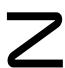
\includegraphics[keepaspectratio]{images/part001_205e3f38.jpg}}

\begin{enumerate}
\def\labelenumi{\arabic{enumi})}
\setcounter{enumi}{1}
\tightlist
\item
  若环 A 不约化为 0 且其仅有的双边理想是 0 与 A，我们有时称 A 是拟单环。若 A 具有一个忠实单模，则称 A 是本原的。由命题 1，每个单环都是拟单环。由于每个非零环都具有一个单模，且单模的零化理想是双边理想，可见每个拟单环都是本原的。然而，存在不是单环的拟单环以及不是拟单环的本原环（VIII, 第 128 页，习题 2）；这样的环不是左阿廷的。
\end{enumerate}

定理 1（韦德伯恩）. —— 一个环是单环当且仅当它同构于一个矩阵环 \(\mathbf{M}_r(\mathrm{D})\)，其中 \(r \geqslant 1\) 是整数，D 是一个体。

引理 1. —— 设 A 是一个单环，S 是一个单左 A-模，D 是体 \(\operatorname{End}_{\mathrm{A}}(\mathrm{S})\) 的反环。那么 S 是一个可逆 (A,D)-双模。它也是 D 上的一个有限维右向量空间，并且映射 \(a \mapsto a_{S}\) 是从 A 到 \(\operatorname{End}_{\mathrm{D}}(\mathrm{S})\) 的环同构。

由命题 1，A-模 \(A_{s}\) 具有有限长度且是 S 型同型的。于是存在一个整数 \(m \geqslant 1\)，使 A-模 \(A_{s}\) 与 \(S^{m}\) 同构。那么 A-模 S 是投射的且有限生成的。它是生成模（VIII, 第 80 页，定理 1），而引理 1 由 VIII, 第 101 页的定理 1 的 (ii)⇒(i) 与 (ii)⇒(iii) 应用于 \((\mathrm{A},\mathrm{D})_{\mathbf{Z}}\)-双模 S 得出。

引理 2. —— 设 D 是一个体，V 是 D 上一个维数有限 \(r \geqslant 1\) 的右向量空间。那么 V 是环 \(\mathrm{E} = \mathrm{End}_{\mathrm{D}}(\mathrm{V})\) 上的单模，且它的交换子等于 \(D_{V}\)。环 E 是单环，其左长度等于 r。

我们知道 V 是一个单 E-模（VIII, 第 45 页，例 3），且其交换子等于 \(D_{V}\)（VIII, 第 82 页，推论 1）。设 \((x_{i})_{1\leqslant i\leqslant r}\) 是 V 在体 D 上的一个基。映射 \(u\mapsto(u(x_{i}))_{1\leqslant i\leqslant r}\) 是从 E-模 \(E_{s}\) 到 E-模 \(V^{r}\) 的同构；于是 E-模 \(E_{s}\) 是长度为 r 的同型模，故环 E 是单环。

现在证明定理 1。回忆（II, §10, No.~7, 第 349 页）环 \(\mathbf{M}_r(\mathrm{D})\) 可以等同于右 D-向量空间 \(\mathrm{D}_d^r\) 的自同态环；此外，体 D 上每个维数为 \(r\) 的右向量空间都同构于 \(\mathrm{D}_d^r\)（II, §7, No.~1, 第 292 页）。于是定理 1 由引理 1 与引理 2 得出。

注 3. —— 设 A 是一个单环，S 是一个单 A-模，D 是体 \(\operatorname{End}_{\mathrm{A}}(\mathrm{S})\) 的反环。那么 A-模 \(A_{s}\) 具有有限长度，且 \(\dim_{\mathrm{D}}(\mathrm{S})\) 等于 \(\operatorname{long}(\mathrm{A})\)。事实上，由引理 1，环 A 同构于 \(\operatorname{End}_{\mathrm{D}}(\mathrm{S})\)；然后应用引理 2 即可。

推论 1. —— a) 单环的中心是一个体。

\begin{enumerate}
\def\labelenumi{\alph{enumi})}
\setcounter{enumi}{1}
\item
  单环的反环是单环。
\item
  单环的左长度等于其右长度。
\end{enumerate}

设 D 是一个体，Z 是它的中心，V 是 D 上一个维数有限 \(r \geqslant 1\) 的右向量空间。我们用 E 表示 V 的自同态环。

由 VIII, 第 83 页的推论 2，映射 \(z \mapsto z_{V}\) 是从 Z 到 E 的中心的同构。断言 a) 得证。V 的对偶 \(V^{*}\) 是 D 的反体 \(D^{o}\) 上的右向量空间，其维数等于 r。映射 \(u \mapsto {}^{t}u\) 是从 E 的反环 \(E^{o}\) 到环 \(\operatorname{End}_{\mathrm{D}^{\circ}}(\mathrm{V}^{*})\) 的同构。于是环 \(E^{o}\) 是单环，且环 E 与 \(E^{o}\) 有相同的左长度，都等于 r（引理 2）。

推论 2. —— 设 r 与 \(r'\) 是严格正的整数，D 与 \(D'\) 是体。环 \(\mathbf{M}_{r}(\mathrm{D})\) 与 \(\mathbf{M}_{r'}(\mathrm{D}')\) 同构当且仅当我们有 \(r = r'\) 且体 D 与 \(D'\) 同构。

该条件显然是充分的。

反之，设环 \(\mathrm{B} = \mathbf{M}_{r}(\mathrm{D})\) 与 \(\mathrm{B}' = \mathbf{M}_{r'}(\mathrm{D}')\) 同构。由于 r 是 \(B_{s}\) 的长度而 \(r'\) 是 \(B'_{s}\) 的长度（引理 2），我们有 \(r = r'\)。此外，B 与 D 森田等价，\(B'\) 与 \(D'\) 森田等价（VIII, 第 102 页，

例 1）。于是体 D 与 D' 是森田等价的，因而同构（VIII, 第 111 页，命题 13, c)）。

推论 3. —— 设 K 是一个交换域（域），A 是一个底环为单环的有限次数 K-代数。存在一个整数 r 与一个 K 上有限次数的 K-代数 D，D 是体，使 A 同构于 \(\mathrm{M}_{r}(\mathrm{D})\)。特别地，若 K 是代数闭的，则 A 同构于 K 上的一个矩阵代数。

设 S 是一个单左 A-模；它是 K 上的一个有限维向量空间。于是它的交换子是 K 上有限次数的代数。从而第一条断言由引理 1 得出。若 K 是代数闭的，则由 VIII, 第 47 页的定理 1 有 D = K。

注 4. —— 设 K 是一个代数闭的交换域（域），A 是 K 上一个有限次数的代数。代数 A 是单的当且仅当存在一个整数 \(n \geqslant 1\)，使 A 同构于 \(\mathrm{M}_{n}(\mathrm{K})\)。此时它的中心同构于 K。

\subsection{单环上的模}

引理 3. —— 设 A 是一个单环，S 是一个单 A-模。用 D 表示 S 的交换子的反体。每个 A-模都同构于形如 \(S \otimes_{D} V\) 的 A-模，其中 V 是体 D 上的一个左向量空间。

这由 VIII, 第 120 页的引理 1 与森田定理（VIII, 第 103 页）得出。

命题 2. —— 设 A 是一个单环，S 是一个单 A-模。

\begin{enumerate}
\def\labelenumi{\alph{enumi})}
\item
  每个 A-模都是投射的且是 S 型同型的，因而是半单的。若它的长度为 a，则它同构于 \(\mathrm{S}^{(a)}\)。
\item
  每个非零 A-模都是生成模。
\item
  两个 A-模同构当且仅当它们有相同的长度。
\end{enumerate}

用 D 表示 S 的交换子的反体。由 VIII, 第 120 页的引理 1，S 是一个可逆 (A,D)-双模。设 M 是一个 A-模；由引理 3，它同构于形如 \(S \otimes_{D} V\) 的模，其中 V 是体 D 上的一个左向量空间。

D-模 V 是投射的且是 \(D_{s}\) 型同型的；它是生成模当且仅当它不约化为 0。最后，\(S \otimes_{D} V\) 的长度等于 D-向量空间 V 的维数，而两个向量空间同构当且仅当它们有相同的维数。于是命题 2 鉴于 VIII, 第 109 页的命题 10 与 VIII, 第 110 页的命题 12 得出。

设 \(r \geqslant 1\) 是一个整数。我们称基数 \(\mathfrak{a}\) 可被 \(r\) 整除，若存在一个基数 \(\mathfrak{b}\) 使 \(\mathfrak{a} = r\mathfrak{b}\)。若 \(\mathfrak{a}\) 是无限的，则情形如此，因为我们有 \(r\mathfrak{a} = \mathfrak{a}\)（《集合论》III, §6, No.~3, 第 188 页，推论 3）。由这一注记推出，若基数 \(\mathfrak{a}\) 可被 \(r\) 整除，则存在唯一的基数 \(\mathfrak{b}\) 使 \(\mathfrak{a} = r\mathfrak{b}\)。

推论. —— 设 k 是一个交换域（域），A 是 k 上一个有限次数的单 k-代数。每个单 A-模在 k 上都是有限维的。两个 A-模同构当且仅当它们在 k 上的维数相等。

每个单 A-模都同构于 \(A_{s}\) 的一个商，因此在 k 上是有限维的。于是该推论由命题 2, c) 得出。

命题 3. —— 设 A 是一个单环。一个 A-模 M 是自由的当且仅当它的长度可被 A 的长度整除。若情形如此，则 M 的所有基都有相同的基数，记作 \(\dim_{\mathrm{A}}(\mathrm{M})\)（II, §7, No.~3, 第 294 页，注 2），它由关系式

\[
\mathrm{long} _ {\mathrm{A}} (\mathrm{M}) = \mathrm{long} (\mathrm{A}) \cdot \mathrm{dim} _ {\mathrm{A}} (\mathrm{M}).\tag{1}
\]

设 M 是自由的，并设 \((e_{i})_{i\in\mathrm{I}}\) 是 M 的一个基。A-模 M 是诸 A-模 \(Ae_{i}\) 的直和，它们各自同构于 \(A_{s}\)。令 \(r=\operatorname{long}_{\mathrm{A}}(\mathrm{A}_{s})\)；这是一个大于或等于 1 的整数（VIII, 第 119 页，命题 1）。由 VIII, 第 73 页的公式 (13)，我们有 \(\operatorname{long}_{\mathrm{A}}(\mathrm{M})=r\operatorname{Card}(\mathrm{I})\)。

反之，设基数 \(\operatorname{long}_{\mathrm{A}}(\mathrm{M})\) 可被 r 整除。设 a 是使 \(\operatorname{long}_{\mathrm{A}}(\mathrm{M}) = r\mathfrak{a}\) 的基数。那么 A-模 M 与 \(\mathrm{A}_{s}^{(\mathfrak{a})}\) 有相同的长度，因而由命题 2 与之同构。这就证明 M 是自由的。

命题 4. —— 设 A 是一个单环，M 是一个非零 A-模。用 B 表示 A-模 M 的自同态环，并把 M 视为一个左 B-模。

\begin{enumerate}
\def\labelenumi{\alph{enumi})}
\item
  映射 \(a \mapsto a_{M}\) 是从 A 到 B-模 M 的自同态环的同构。
\item
  设 M 作为 A-模具有有限长度。那么环 B 是单环，并且我们有
\end{enumerate}

\[
\mathrm{long} _ {\mathrm{A}} (\mathrm{M}) = \mathrm{long} (\mathrm{B}) \text{ 且 } \mathrm{long} _ {\mathrm{B}} (\mathrm{M}) = \mathrm{long} (\mathrm{A}).\tag{2}
\]

由 VIII, 第 122 页的命题 2，A-模 M 是生成模。按定义我们有 \(\mathrm{B} = \mathrm{A}_{\mathrm{M}}'\)，于是断言 a) 由 VIII, 第 82 页的定理 2 得出。

设 M 是一个有限长度的 A-模。选取一个单 A-模 S，并设 D 是其自同态环的反体。由引理 3，A-模 M 同构于形如 \(S \otimes_{D} V\) 的模，其中 V 是体 D 上的一个左向量空间。向量空间 V 是有限维的。由 VIII, 第 64 页的定理 3，环 B 同构于 \(\operatorname{End}_{\mathrm{D}}(\mathrm{V})\)；由引理 2（VIII, 第 121 页），环 B 因而是单环。考虑到 VIII, 第 63 页的注 1，我们得到等式

\[
\mathrm{long(B)} = \mathrm {dim_ {D} (V)} = \mathrm {long_ {A} (M)}.
\]

由 VIII, 第 63 页的注 1 与 VIII, 第 121 页的注 3，我们有关系式

\[
\mathrm{long} _ {\mathrm{B}} (\mathrm{M}) = \mathrm{long} _ {\mathrm{End} _ {\mathrm{D}} (\mathrm{V})} (\mathrm{S} \otimes_ {\mathrm{D}} \mathrm{V}) = \dim_ {\mathrm{D}} (\mathrm{S}) = \mathrm{long} (\mathrm{A}),
\]

由此得最后一个关系式。

\subsection{次数}

考虑一个环 B 与 B 的一个子环 A。给 B 赋以由 \(_{s}B_{d}\) 上的 (B, B)-双模结构经标量限制导出的 (A, A)-双模结构。

命题 5. —— 设 B 是一个环，A 是 B 的一个单子环，S 是一个单左 A-模。那么 B 是一个自由左 A-模，其维数为 \(\text{long}_{\text{A}}(\text{B} \otimes_{\text{A}} \text{S})\)。

设 r 是 A 的长度；A-模 \(A_{s}\) 同构于 \(S^{r}\)。而左 A-模 B 同构于 \(B \otimes_{A} A_{s}\)（II, §3, No.~4, 第 249 页），因而同构于 \((\mathrm{B} \otimes_{\mathrm{A}} \mathrm{S})^{r}\)（II, §3, No.~7, 第 255 页，命题 7）。于是我们有 \(\operatorname{long}_{\mathrm{A}}(\mathrm{B}) = r \operatorname{long}_{\mathrm{A}}(\mathrm{B} \otimes_{\mathrm{A}} \mathrm{S})\)，从而命题 5 由 VIII, 第 123 页的命题 3 得出。

定义 2. —— 设 B 是一个环，A 是 B 的一个单子环。自由左 A-模 B 的维数称为 B 在 A 上的（左）次数，记作 \(^{(1)}\) \([B:A]_{s}\)。

把 A 与 B 换成它们的反环，由上所述可推出 B 是一个自由右 A-模。我们用 \([B : A]_{d}\) 表示它的维数，并称之为 B 在 A 上的右次数。

\pandocbounded{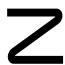
\includegraphics[keepaspectratio]{images/part001_1658b52d.jpg}}

我们可以给出一个体 B 与一个子体 A 的例子，使得次数 \([B:A]_{s}\) 与 \([B:A]_{d}\) 不同。\(^{(2)}\)

设 B 是一个环，A 是 B 的一个单子环，S 是一个单左 A-模。设 M 是一个左 A-模，a 是它的长度。A-模 M 与 \(S^{(a)}\) 同构（VIII, 第 122 页，命题 2），因而 B-模 \(B \otimes_{A} M\) 与 \((\mathrm{B} \otimes_{\mathrm{A}} \mathrm{S})^{(a)}\) 亦然。关系式

\[
\mathrm{long} _ {\mathrm{A}} (\mathrm{B} \otimes_ {\mathrm{A}} \mathrm{M}) = [ \mathrm{B}: \mathrm{A} ] _ {s} \mathrm{long} _ {\mathrm{A}} (\mathrm{M})\tag{3}
\]

由命题 5 与定义 2 得出。

命题 6. —— 设 C 是一个环，B 是 C 的一个单子环，A 是 B 的一个单子环。那么我们有 \([C:A]_{s} = [C:B]_{s}[B:A]_{s}\)。

引入把 C 视为左 B-模时的一个基 \((e_{i})_{i\in\mathrm{I}}\)，以及把 B 视为左 A-模时的一个基 \((f_{j})_{j\in\mathrm{J}}\)。那么族 \((f_{j}e_{i})_{j\in\mathrm{J},i\in\mathrm{I}}\) 是把 C 视为左 A-模时的一个基（II, §1, No.~13, 第 222 页，命题 25）；命题 6 得证。

注. —— 1) 设 A 是单环 B 的一个单子环，且右次数 \([B : A]_{d}\) 有限。设 C 是把 B 视为右 A-模时的自同态环；由 VIII, 第 123 页的命题 4, b)，它是一个单环。对 B 中的任意 b，设 \(\gamma(b)\) 是从 B 到 B 的映射 \(x \mapsto bx\)；则 \(\gamma : b \mapsto \gamma(b)\) 是从 B 到 C 的一个子环的同构。此外，若 \((x_{1}, \ldots, x_{m})\) 是右 A-模 B 的一个基，则把 c 映为 \((c(x_{1}), \ldots, c(x_{m}))\) 的态射是从 C 到 \(B_{s}^{m}\) 的左 B-模同构；于是我们有关系式

\[
[ \mathrm{C}: \gamma (\mathrm{B}) ] _ {s} = [ \mathrm{B}: \mathrm{A} ] _ {d}.\tag{4}
\]

把 VIII, 第 123 页的关系式 (2) 应用于右 A-模 B，我们看出

\[
\mathrm{long} (\mathrm{C}) = [ \mathrm{B}: \mathrm{A} ] _ {d} \mathrm{long} (\mathrm{A}).\tag{5}
\]

\begin{enumerate}
\def\labelenumi{\arabic{enumi})}
\setcounter{enumi}{1}
\tightlist
\item
  设 \(\mathrm{K}\) 是一个交换域（域）。若 \(\mathrm{A}\) 是有限次数代数 \(\mathrm{B}\)（在 \(\mathrm{K}\) 上）的一个单子代数，则由 VIII, 第 125 页的命题 6，\(\mathrm{B}\) 在 \(\mathrm{A}\) 上的左次数满足关系式 \(\left[\mathrm{B}:\mathrm{A}\right]_s[\mathrm{A}:\mathrm{K}] = [\mathrm{B}:\mathrm{K}]\)。同样，我们有 \(\left[\mathrm{B}:\mathrm{A}\right]_d[\mathrm{A}:\mathrm{K}] = [\mathrm{B}:\mathrm{K}]\)。由此得等式 \(\left[\mathrm{B}:\mathrm{A}\right]_s = \left[\mathrm{B}:\mathrm{A}\right]_d\)。
\end{enumerate}

\subsection{单环的理想}

设 D 是一个体，V 是 D 上一个维数有限 \(n \geqslant 1\) 的右向量空间。考虑单环 \(A = \text{End}_{\text{D}}(\text{V})\)。对 V 的每个线性子空间 W，把 A 中满足 \(aW = 0\)（相应地，\(aV \subset W\)）的元素 a 之集记作 \(\mathfrak{a}(\text{W})\)（相应地，\(\mathfrak{b}(\text{W})\)）。

命题 7. —— a) 映射 \(W \mapsto \mathfrak{a}(W)\) 是从 V 的线性子空间之集到 A 的左理想之集的双射。

\begin{enumerate}
\def\labelenumi{\alph{enumi})}
\setcounter{enumi}{1}
\item
  映射 \(W \mapsto \mathfrak{b}(W)\) 是从 V 的线性子空间之集到 A 的右理想之集的双射。
\item
  设 \(\mathrm{W}_1\) 与 \(\mathrm{W}_2\) 是 \(\mathrm{V}\) 的线性子空间。关系 \(\mathrm{W}_1 \subset \mathrm{W}_2\)、\(\mathfrak{a}(\mathrm{W}_1) \supset \mathfrak{a}(\mathrm{W}_2)\) 与 \(\mathfrak{b}(\mathrm{W}_1) \subset \mathfrak{b}(\mathrm{W}_2)\) 等价。
\end{enumerate}

断言 b) 由把 VIII, 第 104 页的例 1, b) 应用于可逆 \((\mathrm{D}^{\circ},\mathrm{A}^{\circ})\)-双模 V 得出，关系 \(\mathrm{W}_1\subset \mathrm{W}_2\) 与 \(\mathfrak{b}(\mathrm{W}_1)\subset \mathfrak{b}(\mathrm{W}_2)\) 的等价性亦然。

设 \(V^{*}\) 是 V 的对偶，视为 D 的反体 \(D^{\circ}\) 上的右向量空间。对 V 的每个子空间 W，把 W 在 \(V^{*}\) 中的正交子空间记作 \(W'\)。映射 \(W \mapsto W'\) 是从 V 的子空间之集到 \(V^{*}\) 的子空间之集的双射。若 \(W_{1}\) 与 \(W_{2}\) 是 V 的两个子空间，则关系 \(W_{1} \subset W_{2}\) 与 \(W_{1}' \supset W_{2}'\) 等价。而映射 \(u \mapsto {}^{t}u\) 是从 A 到 \(\operatorname{End}_{D^{\circ}}(V^{*})\) 的反环的同构；它把 A 的左理想变为 \(\operatorname{End}_{D^{\circ}}(V^{*})\) 的右理想，并把 \(\mathfrak{a}(W)\) 变为 \(\mathfrak{b}(W')\)，即 \(V^{*}\) 的满足 \(h(V^{*}) \subset W'\) 的自同态 h 之集。于是断言 a) 以及关系 \(W_{1} \subset W_{2}\) 与 \(\mathfrak{a}(W_{1}) \supset \mathfrak{a}(W_{2})\) 的等价性，由关于 V 的对偶 \(V^{*}\) 的与 b) 类似的断言得出。

推论. —— a) A 的极小左理想是诸理想 \(\mathfrak{a}(\mathrm{H})\)，其中 H 是 V 的一个超平面。A 的极大左理想是诸理想 \(\mathfrak{a}(\mathrm{L})\)，其中 L 是 V 的一条直线。

\begin{enumerate}
\def\labelenumi{\alph{enumi})}
\setcounter{enumi}{1}
\tightlist
\item
  A 的极小右理想是诸理想 \(\mathfrak{b}(\mathrm{L})\)，其中 L 是 V 的一条直线。A 的极大右理想是诸理想 \(\mathfrak{b}(\mathrm{H})\)，其中 H 是 V 的一个超平面。
\end{enumerate}

设 \((\mathrm{L}_{i})_{i\in\mathrm{I}}\) 是一族直和为 V 的直线。设 \((\varepsilon_{i})_{i\in\mathrm{I}}\) 是与分解 \(V=\oplus_{i\in\mathrm{I}}L_{i}\) 相伴的投影算子族。诸 \(\varepsilon_{i}\) 是 A 中的幂等元，并且我们有 \(\varepsilon_{i}\varepsilon_{j} = 0\)（对 \(i\neq j\)）且 \(\sum_{i\in \mathrm{I}}\varepsilon_i = 1\)。把超平面 \(\sum_{j\neq i}\mathrm{L}_j\) 记作 \(\mathrm{H}_i\)；它是 \(\varepsilon_{i}\) 的核。于是我们有

\[
\mathfrak {a} (\mathrm{H} _ {i}) = \mathrm{A}   \varepsilon_ {i}  , \quad \mathfrak {b} (\mathrm{L} _ {i}) = \varepsilon_ {i}   \mathrm{A}  .
\]

A-模 \(A_{s}\) 是极小左理想族 \((\mathfrak{a}(\mathrm{H}_{i}))_{i\in\mathrm{I}}\) 的直和，而 \(A_{d}\) 是极小右理想族 \((\mathfrak{b}(\mathrm{L}_{i}))_{i\in\mathrm{I}}\) 的直和。

考虑特殊情形 \(V = D_{d}^{n}\)，并把 A 等同于矩阵环 \(\mathbf{M}_{n}(\mathrm{D})\)。用 I 表示 N 中的区间 \([1, n]\)，用 \((v_{i})_{i \in \mathrm{I}}\) 表示 V 的典范基；令 \(L_{i} = v_{i}D\)，并用 \(E_{ij}\) 表示矩阵单位（II, §10, No.~3, 第 341 页）。于是我们有 \(\varepsilon_{i} = E_{ii}\)。左理想 \(AE_{ii}\) 等于 \(DE_{1i} + \cdots + DE_{ni}\)，由除第 i 列外所有列均为零的矩阵组成。右理想 \(E_{ii}A\) 等于 \(DE_{i1} + \cdots + DE_{in}\)，由除第 i 行外所有行均为零的矩阵组成。我们还有关系式

\[
\mathrm{E} _ {i i} \mathrm{AE} _ {j j} = \mathrm{E} _ {i i} \mathrm{A} \cap \mathrm{AE} _ {j j} = \mathrm{DE} _ {i j}
\]

其中 i 与 j 介于 1 与 n 之间。
